\documentclass[letterpaper,11pt]{scrreprt}
\usepackage[american]{babel}
\usepackage[latin1]{inputenc}
\usepackage[T1]{fontenc}
\usepackage[top=1in,bottom=1in,left=1in,right=1in]{geometry}
\usepackage{lmodern}

\usepackage{amsmath}
\usepackage{amssymb}

\usepackage[hyperref]{ntheorem}
\usepackage[
	bookmarks,
	colorlinks=false,
	linkcolor=blue,
	citecolor=blue,
	pagebackref=false,
	pdftitle={MADlib Design Document},
	pdfauthor={Predictive Analytics Team, Pivotal Inc.},
	pdfsubject={},
	pdfkeywords={}
]{hyperref}
\usepackage{csquotes}                  % Strongly recommended for biblatex
\usepackage[
	backend=bibtex,
	maxnames=2,
	maxbibnames=20,
	firstinits=true
]{biblatex}
\usepackage{scrpage2}                  % Headers and footers
\usepackage{color}                     % Colors, possibly only for \todo
\usepackage{enumitem}                  % enumerate environment
\usepackage{ctable}
\usepackage{tabularx}
\usepackage{xspace}                    % Correct spaces after \newcommand definitions
\usepackage[noend]{algpseudocode}      % algorithm environment
\usepackage{listings}                  % Code snippets
\usepackage{bbding}
\usepackage{latex/tikz-uml}            % UML diagrams

% BEGIN Doc Layout
	\allowdisplaybreaks[3]

	\pagestyle{scrheadings}
	\automark[chapter]{section}

	\setkomafont{disposition}{\normalcolor\bfseries}
	\setkomafont{descriptionlabel}{\bfseries}
	\setkomafont{captionlabel}{\usekomafont{disposition}}

	\setlength{\arrayrulewidth}{.5pt}
	\numberwithin{equation}{section}
	\renewcommand{\theenumi}{\roman{enumi}}
	\renewcommand{\labelenumi}{\theenumi)}

	\newcommand{\otoprule}{\midrule[\heavyrulewidth]}

	\setcounter{secnumdepth}{3}

	\makeatletter
	% Algorithms are expected to have an optional argument of form
	% FunctionName$(ArgumentList)$, e.g., DiscreteSample$(A, w)$
	\def\internal@funcName#1$(#2)${#1}
	\newcommand\funcName[1]{\internal@funcName #1}
	\newtheoremstyle{algorithm}
		{\item[\rlap{\vbox{\hbox{\hskip\labelsep \theorem@headerfont
			##1\ ##2\theorem@separator}\hbox{\strut}}}]}%
		{\item[\rlap{\vbox{\hbox{\hskip\labelsep {\theorem@headerfont
			##1}\ \normalfont\texttt{##3}{\theorem@headerfont\theorem@separator}}\hbox{\strut}}}]%
			\def\@currentlabel{\texttt{\funcName{##3}}}}
	\makeatother

	\makeatletter
	% Also display JSTOR in small caps
	% http://sourceforge.net/tracker/index.php?func=detail&aid=3152938&group_id=244752&atid=1126006
	\DeclareFieldFormat{eprint:arxiv}{%
	  \textsc{arXiv}\addcolon
	  \ifhyperref
	    {\href{http://arxiv.org/\abx@arxivpath/#1}{%
	       \nolinkurl{#1}%
	       \iffieldundef{eprintclass}
		 {}
		 {\addspace\texttt{\mkbibbrackets{\thefield{eprintclass}}}}}}
	    {\nolinkurl{#1}
	     \iffieldundef{eprintclass}
	       {}
	       {\addspace\texttt{\mkbibbrackets{\thefield{eprintclass}}}}}}
	\DeclareFieldFormat{eprint:jstor}{%
	  \mkbibacro{JSTOR}\addcolon\space
	  \ifhyperref
	    {\href{http://www.jstor.org/stable/#1}{\nolinkurl{#1}}}
	    {\nolinkurl{#1}}}
	% Some conferences do not have DOIs for their papers, but they do get
	% IDs in the ACM Digital Library. E.g., SODA papers.
	\DeclareFieldFormat{eprint:acm}{%
	  \mkbibacro{ACM}\addcolon\space
	  \ifhyperref
	    {\href{http://dl.acm.org/citation.cfm?id=#1}{\nolinkurl{#1}}}
	    {\nolinkurl{#1}}}
	\makeatother

	\newlist{moduleinfo}{description}{2}
	\setlist[moduleinfo]{style=multiline,labelindent=\leftmargini,leftmargin=3cm,rightmargin=\leftmargini,font=\bfseries}
	\newlist{modulehistory}{description}{2}
	\setlist[modulehistory]{style=multiline,leftmargin=1.1cm}
% END Doc Layout

% BEGIN General Definitions
	\newcommand{\todo}[1]{\textbf{\color{red}#1}}

	\newcommand{\specialcell}[3][t]{%
		\begin{tabular}[#1]{@{}#2@{}}#3\end{tabular}}

	% BEGIN Mathematical Definition
		% Space (only) in displaymath (e.g., between mathematical expression and punctuation mark)
		\newcommand{\SiM}{\mathchoice{\,}{}{}{}}
	% END Mathematical Operators

	% BEGIN URLs
		\newcommand{\mailto}[1]{\href{mailto:#1}{\nolinkurl{#1}}}
		\newcommand{\doi}[1]{DOI: \href{http://dx.doi.org/#1}{\nolinkurl{#1}}}
	% END URLs

	\makeatletter
	% BEGIN Mathematical Definitions
		% BEGIN Set Symbols
			\newcommand{\setsymbol}[1]{\mathbb{#1}}
			\newcommand{\N}{\@ifstar{\setsymbol{N}_0}{\setsymbol{N}}}
			\newcommand{\R}{\setsymbol{R}}
		    \newcommand{\Nupto}{\@ifstar{\Nupto@star}{\Nupto@nostar}}
		    \newcommand{\Nupto@star}[1]{[#1]_0}
		    \newcommand{\Nupto@nostar}[1]{[#1]}
		% END Set Symbols
		\renewcommand{\vec}[1]{\ensuremath{\boldsymbol{#1}}}
	% END Mathematical Definitions
	\makeatother

	\renewcommand{\vec}[1]{\ensuremath{\boldsymbol{#1}}}
	\newcommand{\enumref}[1]{(\ref{#1})}

	\makeatletter
	\newcommand{\symlabel}[2]{\def\@currentlabel{\texttt{#1}}\texttt{#1}\label{#2}}
	\makeatother

	\newcommand{\Warning}[1]{\marginpar[\HandRight]{\HandLeft}\textbf{#1}}

	% BEGIN Algorithms
	\theoremstyle{algorithm}
	\theorembodyfont{\upshape}
	\newtheorem{algorithm}{Algorithm}[section]

	\newlength{\alglabelwidth}
	\newcommand{\alginput}[1]{%
		\par\noindent%
		\settowidth{\alglabelwidth}{\emph{Output:}}%
		\makebox[\alglabelwidth][l]{\emph{Input:}} \begin{tabular}[t]{l} #1 \end{tabular}}
	\newcommand{\algoutput}[1]{%
		\par\noindent%
		\settowidth{\alglabelwidth}{\emph{Output:}}%
		\makebox[\alglabelwidth][l]{\emph{Output:}} \begin{tabular}[t]{l} #1 \end{tabular}}
	\newcommand{\algprecond}[1]{%
		\par\noindent\textit{Initialization/Precondition: #1}}

	\newcommand{\set}{\leftarrow}
	\DeclareMathOperator{\random}{random}
	\newcommand{\dist}{\ensuremath{\mathit{dist}}}
	\newcommand{\List}{\mathrm{List}}
	\newcommand{\Sample}{\mathit{Sample}}
	\algblockdefx[With]{With}{EndWith}%
		[1]{\textbf{with} #1 \textbf{do}}%
		[0]{End}
	\algnotext[With]{EndWith}
	% END Algorithms

	% BEGIN lstlisting environments
	\lstset{
		basicstyle=\ttfamily\footnotesize,       % the size of the fonts that are used for the code
		numbers=left,                   % where to put the line-numbers
		numberblanklines=false
		numbersep=1em,                  % how far the line-numbers are from the code
		basewidth=0.52em,
		tabsize=4,  		% sets default tabsize to 2 spaces
		xleftmargin=\leftmargini
	}
	\renewcommand*\thelstnumber{\the\value{lstnumber}:}
	% END lstlisting environments

	\lstnewenvironment{sql}[1][]{\lstset{language=SQL,gobble=4,emphstyle=\textit,#1}}{}
	\lstnewenvironment{cpp}[1][]{\lstset{language=C++,gobble=4,emphstyle=\textit,#1}}{}
	\lstnewenvironment{cppsnippet}[1][]{\lstset{basicstyle=\ttfamily,language=C++,stepnumber=0,gobble=8,emphstyle=\textit,xleftmargin=0pt,#1}}{}
% END General Definitions

\bibliography{../literature.bib}

% BEGIN Preamble
\title{%
	MADlib Design Document%
}

\newcommand{\bR}{\mathcal{R}}
\newcommand{\norm}[1]{\| #1 \|_2}


\begin{document}

\maketitle

\tableofcontents

\input{other-chapters/abstraction-layers}
\input{modules/sampling}
\input{modules/matrix-operations}
\chapter[Linear Systems]{Linear Systems}
\begin{moduleinfo}
\item[Authors] {Srikrishna Sridhar}
\item[History]
	\begin{modulehistory}
		\item[v1.0] Initial version
	\end{modulehistory}
\end{moduleinfo}

\section{Introduction}\label{sec:intro}
In this document, we describe solution methods for systems of a consistent
linear equations.
\begin{equation}
  \label{eq:linear_system}
  Ax = b
\end{equation}
where $x \in \R^{n}$, $A \in \R^{m \times n}$ and $b \in \R^{m}$. We assume
that all rows of $A$ are non-zero. We denote the rows of $A$ and $b$
by $a^T_i$ and $b_i$, respectively. This can be written
as
\begin{alignat}{2}
A &= \begin{bmatrix} a^T_1 \  a^T_2  \  \ldots \  a^T_m   \end{bmatrix} \ \ \ \
b &&= \begin{bmatrix} b_1  \  b_2   \ \ldots \  b_m   \end{bmatrix}
\end{alignat}

The algorithms discussed in this document are suitable for large sparse
linear systems which are expensive for ordinary elimination. Amongst the many methods for
iteratively solving linear systems, algorithms like the Jacobi and over-relaxation
methods not as effective as methods like conjugate gradient. The preconditioned
conjugate gradient (CG) method is one of the most commonly used algorithms for
solving large sparse systems for symmetric $A$. The textbook CG algorithm has been modified
to be applicable even when $A$ is not symmetric. The disadvantage of CG is that
in each iteration, it must perform a matrix-vector product. To avoid this computation,
some applications implement a new algorithm called the randomized Kaczmarz (RK)
algorithm. It is a popular choice for extremely large scale applications.
The algorithm is known to have a linear convergence rate and each iteration
requires an $O(n)$ operation. In some applications, it outperforms CG. In
general, it is be difficult to predict which one of CG or RK is preferable
for a given linear system.

We now discuss three different approaches to solve linear systems. Direct method,
Conjugate Gradient and Randomized Kaczmarz. Each method has its own advantages
and disadvantages which will be highlighted.

\section{Direct Methods}
Direct methods are suitable for solving small linear systems that fit completely
in memory. The workhorse of several commercial codes is the LU decomposition.
The LU decomposition factors a matrix as the product of a lower triangular matrix
($L$) and an upper triangular matrix ($U$) such that
$$
PA = LU
$$
where $P$ is a permutation matrix which re-orders the rows of $A$. Such an
LU-decomposition can be used to solve \eqref{eq:linear_system} using
$$
  Ax = b \Rightarrow LUx = Pb
$$

Now, we can solve for $x$ using the following steps
\begin{enumerate}
  \item Solve for $y$ in the equation $Ly = Pb$
  \item Solve for $x$ in the equation $Ux = b$
\end{enumerate}
Since both $L$ and $U$ are triangular matrices, we can efficiently solve both
the equations directly using forward and backward substitutions.

The main advantage of solving linear systems with direct methods is that direct
methods are independent of the conditioning of the system. Solve time depends
purely on the sparsity and size of the matrices. The major disadvantage is
that the LU-decomposition has large memory requirements. Even when the matrix
$A$ is sparse, the $L$ and $U$ factors might be dense. The large memory
requirements make it unsuitable for solving large or very sparse linear
systems.

\section{Iterative Methods}
In solving \eqref{eq:linear_system} a convergent iterative method starts
with an initial estimate $x_0$ of the solution and generates a sequence of iterates
$x_k$ that are successively closer to the solution $x^*$. Iterative methods
are often useful even for linear problems involving a large number of variables.
Amongst the many iterative methods, we will review the two most popular methods;
the conjugate gradient method (CG) and the randomized Kaczmarz (RK) method.

\subsection{Conjugate Gradient (CG)}
The linear conjugate gradient method (not to be confused with the non-linear
conjugate gradient method) to solve large sparse linear systems with a
{\it symmetric positive definite} $A$ matrix. Such a system can be stated as:
\begin{equation}
  \label{eq:sym_linear_system}
  Ax = b
\end{equation}
where $x \in \R^{n}$, $A \in \R^{n \times n}$ is symmetric and positive
definite and $b \in \R^{n}$.

Unlike direct methods, the time taken to solve a linear system using CG depends on the
distribution of the eigenvalues of the $A$ matrix. In some applications,
the $A$ matrix is appropriately scaled by a process called pre-conditioning to
generate an equivalent system with a more favorable distribution of eigenvalues.


The system \eqref{eq:sym_linear_system} can be restated as the quadratic minimization
$$
  \min \phi(x) := \frac{1}{2} x^T A^T A x - b^T x
$$
which allows us to interpret CG as an algorithm to minimize convex quadratic
functions. In the rest of this section, we will refer to the gradient $\nabla \phi(x)$
as the residual of the linear system:
$$
  \nabla \phi(x) := r(x) := Ax - b
$$
The linear conjugate gradient method generates a sequence of directions ${p_0, p_1 \ldots p_l}$
that satisfy an important property called conjugacy which implies that the method
can minimize the function $\phi(x)$ in exactly $n$ steps. We refer the reader
to the textbook by Nocedal and Wright \cite{nocedal2006numerical} for details on the
theoretical and algorithmic aspects of CG.

We now discuss an efficient implementation of the linear CG algorithm. In each,
iteration ($k$), we keep track of the direction vector $p_k$, the residual
vector $r_k$ and the solution vector $x_k$. The computational bottleneck
is in a matrix-vector multiplication between $A$ and $p$.

\begin{algorithm}%
% [Conjugate gradient for symmetric positive definite linear systems]
% \caption{Conjugate gradient for symmetric positive definite linear systems.}\label{alg:cg}
\alginput{Symmetric matrix $A \in \R{m \times n}$, $b \in \R{m}$}
\algoutput{Solution to $Ax=b$}
\begin{algorithmic}[1]
  \State Choose $x_0 \in \R^n$, $r_0 \leftarrow Ax_0$, $p_0 \leftarrow -r_0$, $k \leftarrow 0$
  \While{$\norm{r_k} \leq \epsilon$}
    \State$z_k \leftarrow Ap_k$
    \State$\alpha_k \leftarrow \frac{r_k^T r_k}{p_k^T z_k}$
    \State$x_{k+1} \leftarrow x_k + \alpha_k p_k$
    \State$r_{k+1} \leftarrow r_k + \alpha_k z_k$
    \State$\beta_k \leftarrow \frac{r_{k+1}^T r_{k+1}}{r_k^T r_k}$
    \State$p_{k+1} \leftarrow -r_{k+1} + \beta_{k+1} p_k$
    \State$k = k + 1$
  \EndWhile
\end{algorithmic}
\label{alg:cg}
\end{algorithm}

The conjugate gradient method is suitable for large sparse linear systems where
direct methods can often run into memory bottlenecks. This is mainly because,
the only memory requirements of the CG method is to store the latest copies
of the vectors $p_k$, $r_k$ and $x_k$. The majority of the computational efforts
are spent in the step $z_k \leftarrow A p_k$. Hence, CG tends to perform better
in sparse linear systems.

\subsubsection*{Conjugate gradient Least Squares (CGLS)}
In this section, we will extend the CG algorithm to be numerically suited to any linear system of the form
\eqref{eq:linear_system}. The naive extension of CG to \eqref{eq:sym_linear_system}
solves $A^TAx = A^Tb$. In addition to requiring an expensive matrix-matrix
multiplication algorithm, it has it use of vectors of the form $A^TAp$. An
algorithm with better numerical properties was developed by Hestenes et. al \cite{hestenes1952methods}.


\begin{algorithm}
% \caption{Conjugate Gradient (least squares) for general linear systems.} \label{alg:cgls}
\alginput{Matrix $A \in \R{m \times n}$, $b \in \R{m}$}
\algoutput{Solution to $Ax=b$}
\begin{algorithmic}[1]
\State Choose $x_0 \in \R^n$, $r_0 \leftarrow b$,\ $s_0 \leftarrow A^Tb$, $p_0 \leftarrow s_0$, $\gamma_0=\norm{s_0}^2$, $k \leftarrow 0$
\While{$\norm{r_k} \leq \epsilon$}
  \State$z_k \leftarrow Ap_k$
  \State$\alpha_k \leftarrow \frac{\gamma_{k}}{z_k^Tz_k}$
  \State$x_{k+1} \leftarrow x_k + \alpha_k p_k$
  \State$r_{k+1} \leftarrow r_k - \alpha_k z_k$
  \State$s_{k+1} \leftarrow A^T r_{k+1} $
  \State$\gamma_{k+1} \leftarrow s_{k+1}^T s_{k+1}$
  \State$\beta_{k+1} \leftarrow \frac{\gamma_{k+1}}{\gamma_k}$
  \State$p_{k+1} \leftarrow s_{k+1} + \beta_{k+1} p_k$
  \State$k = k + 1$
\EndWhile
\end{algorithmic}
\label{alg:cgls}
\end{algorithm}

Paige et. al \cite{paige1982lsqr} developed an algorithm called LSQR which has similar performance
to CGLS. We might consider implementing LSQR in case CG performs poorly on
linear systems.

\subsection{Randomized Kaczmarz (RK)}
As discussed earlier, the randomized Kaczmarz (RK) algorithm, is a popular
algorithm for solving \eqref{eq:linear_system}. Each iteration requires an
$O(n)$ storage and computational effort. During each iteration, RK picks a
row $a_i$ of the matrix $A$, and does an orthogonal projection of the current
solution vector $x_k$ to the hyperplane $a_i^Tx = b$. The update step is given by
$$
x_{k+1} = x_k - \frac{(a_i^T x_k - b_i)}{\norm{a_i}} a_i
$$
An alternate interpretation of RK is that the algorithm is identical to the
stochastic gradient  descent algorithm on the problem
$$
  \min \phi(x) := \frac{1}{2} x^T A^T A x - b^T x
$$
The algorithm performs best when a row $i$ is chosen randomly but proportional
to $\norm{a_i}$. Since sequential scans are preferred for in-database algorithms,
a common pre-processing procedure for RK is to rescale the system so that each
equation $a_i^Tx = b$ has the same norm.

\begin{algorithm}%[Randomized Kaczmarz for general linear systems]
% \caption{Randomized Kaczmarz for general linear systems.}\label{alg:rk}
\alginput{Matrix $A \in \R{m \times n}$, $b \in \R{m}$}
\algoutput{Solution to $Ax=b$}
\begin{algorithmic}[1]
\State Choose $x_0 \in \R^n$, $k \leftarrow 0$
\While{$\norm{Ax - b} \leq \epsilon$}
\State$x_{k+1} \leftarrow x_k - \frac{(a_i^T x_k - b_i)}{\norm{a_i}}$
  \State$k = k + 1$
\EndWhile
\end{algorithmic}
\label{alg:rk}
\end{algorithm}

The termination criterion of the algorithm is implemented by computing the
residual $\norm{Ax-b}$ extremely infrequently. Typically, this computation
is performed every $K$ epochs where an epoch is defined as one whole pass of
the data which in the case of RK is $m$ iterations.

% When using TeXShop on the Mac, let it know the root document. The following must be one of the first 20 lines.
% !TEX root = ../design.tex

\chapter[Singular Value Decomposition]{Singular Value Decomposition}

\begin{moduleinfo}
\item[Author] \href{mailto:riyer@gopivotal.com}{Rahul Iyer}
\item[History]
    \begin{modulehistory}
        \item[v0.1] Initial version
    \end{modulehistory}
\end{moduleinfo}

\newcommand{\vectornorm}[1]{\left|\left|#1\right|\right|}
\def\Rset{\mathbb{R}}
% Abstract. What is the problem we want to solve?
In linear algebra, the singular value decomposition (SVD) is a factorization of
a real or complex matrix, with many useful applications in signal processing and
statistics.

Let $A$ be an $m \times n$ matrix, where $m \ge n$. Then $A$ can be decomposed as follows:
\begin{gather*}
    A = U \Sigma V^T,
\end{gather*}
where $U$ is a $m \times n$ orthonormal matrix, $\Sigma$ is a $n\times n$
diagonal matrix, and $V$ is an $n\times n$ orthonormal matrix. The diagonal
elements of $\Sigma$ are called the \emph{singular values}.

It is possible to formulate the problem of computing the singular triplets
($\sigma_i, u_i, v_i$) of $A$ as an eigenvalue problem involving a Hermitian
matrix related to $A$. There are two possible ways of achieving this:

\begin{figure}[tb]
    \begin{center}
        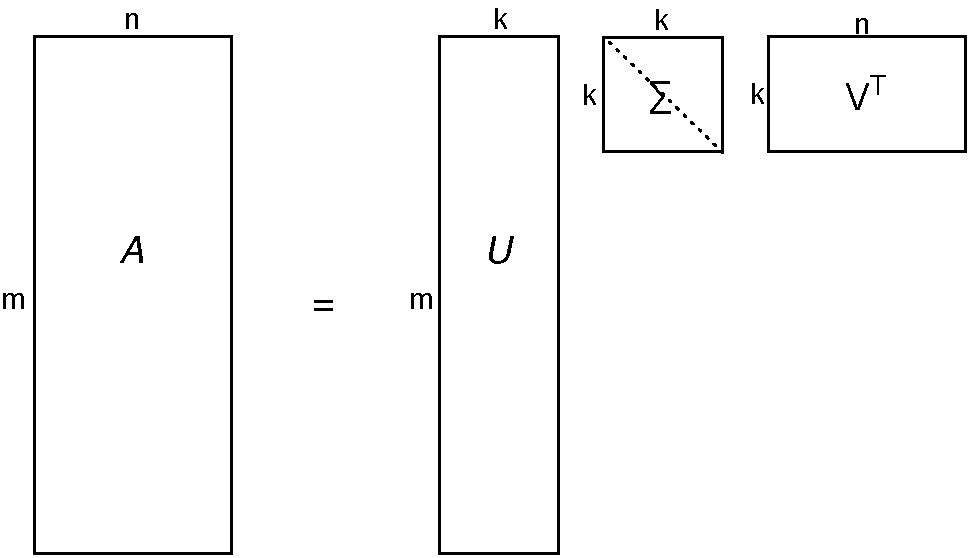
\includegraphics[width=\textwidth]{figures/svd_figure}
    \end{center}
    \caption{Singular Value Decomposition}
    \label{fig:svd}
\end{figure}

\begin{enumerate}
    \item With the cross product matrix, $A^TA$ and $AA^T$
    \item With the cyclic matrix $H(A) =
        \begin{bmatrix}
            0   & A\\
            A^* & 0
        \end{bmatrix}$
\end{enumerate}

The singular values are the nonnegative square roots of the eigenvalues of the
cross product matrix. This approach may imply a severe loss of accuracy in the
smallest singular values. The cyclic matrix approach is an alternative that
avoids this problem, but at the expense of significantly increasing the cost of
the computation.

Computing the cross product matrix explicitly is not recommended, especially in
the case of sparse A. Bidiagonalization was proposed by Golub and
Kahan~\cite{golub1965} as a way of tridiagonalizing the cross product matrix
without forming it explicitly.

Consider the following decomposition
\begin{gather*}
    A = P B Q^T,
\end{gather*}

where P and Q are unitary matrices and B is an $m\times n$ upper bidiagonal
matrix. Then the tridiagonal matrix $BB^T$ is unitarily similar to $AA^T$.
Additionally, specific methods exist that compute the singular values of $B$
without forming $BB^T$. Therefore, after computing the SVD of B,
\begin{gather*}
    B = X \Sigma Y^T,
\end{gather*}
it only remains to compute the SVD of the original matrix with $U = PX$ and $V = QY$.

\section{Lanczos Bidiagonalization} % (fold)
\label{sec:lanczos_bidiagonalization}

The Lanczos algorithm is an iterative algorithm devised by Cornelius Lanczos
that is an adaptation of power methods to find eigenvalues and eigenvectors of a
square matrix or the singular value decomposition of a rectangular matrix. It is
particularly useful for finding decompositions of very large sparse matrices.

For a rectangular matrix $A$, the Lanczos bidiagonalization method computes a
sequence of Lanczos vectors $p_j \in \mathbb{R}^m$ and $q_j \in \mathbb{R}^n$
and scalars $\alpha_j$ and $\beta_j$ for $j = 1, 2, \ldots, k$ as follows:

\begin{algorithm}[Lanczos Bidiagonalization Algorithm]
 % \label{alg:lanczos-bidiagonalization}
\begin{algorithmic}[1]
     \State Choose a unit-norm vector $q_1$ and let $\beta_0 = 0$ and $p_0 = 0$
     \For{$j = 1, 2, \ldots, k$}
        \State $p_j \set Aq_j - \beta_{j-1} p_{j-1}$
        \State $\alpha_j \set \vectornorm{p_j}_2$
        \State $p_j \set p_j/\alpha_j$
        \State $q_{j+1} \set A^Tp_j - \alpha_j q_j$
        \State $\beta_j \set \vectornorm{q_{j+1}}_2$
        \State $q_{j+1} \set q_{j+1}/\beta_j$
    \EndFor
\end{algorithmic}
\end{algorithm}


After $k$ steps, we can generate the bidiagonal matrix $B_k$ as follows,
\[
\begin{bmatrix}
    \alpha_1    & \beta_1   &           &           &               & \\
                & \alpha_2  & \beta_2   &           &               & \\
                &           & \alpha_3  & \beta_3   &               & \\
                &           &           & \ddots    & \ddots        & \\
                &           &           &           & \alpha_{k-1}  & \beta_{k-1} \\
                &           &           &           &               & \alpha_k
\end{bmatrix}
\]
In exact arithmetic the Lanczos vectors are orthonormal such that,
\begin{gather*}
    P_{k+1} = (p_1, p_2, \dotsc, p_{k+1}) \in \mathbb{R}^{m \times (k+1)},
        P_{k+1}^T P_{k+1} = I_{k+1} \\
    Q_{k+1} = (q_1, q_2, \dotsc, q_{k+1}) \in \mathbb{R}^{n \times  (k+1)},
        Q_{k+1}^T Q_{k+1} = I_{k+1}.
\end{gather*}

\begin{figure}[tb]
    \centering
        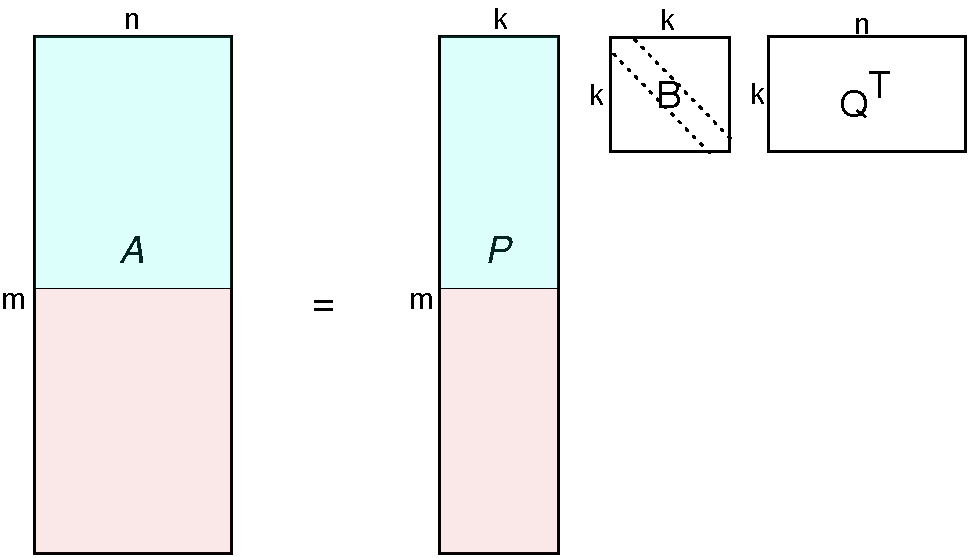
\includegraphics[width=\textwidth]{figures/lanczos_bidiag_segment}
    \caption{Lanczos bidiagonalization of $A$}
    \label{fig:lanczos}
\end{figure}
After $k$ Lanczos steps, the Ritz values $\tilde{\sigma_i}$ (approximate singular
values of A) are equal to the computed singular values of $B_k$, and the
Ritz vectors are
\begin{gather*}
    \tilde{u_i} = P_k x_i,  \qquad  \tilde{v_i} = Q_k y_i
\end{gather*}
% subsubsection lanczos_bidiagonalization (end)

\section{Dealing with Loss of Orthogonality} % (fold)
\label{sec:dealing_with_loss_of_orthogonality}

After a sufficient number of steps the Lanczos vectors start to lose their
mutual orthogonality, and this happens together with the appearance in the
spectrum of $B_j$ of repeated and spurious Ritz values. The simplest cure for
this loss of orthogonality is full orthogonalization. In Lanczos
bidiagonalization, two sets of Lanczos vectors are computed, so full
orthogonalization amounts to orthogonalizing vector $p_j$ explicitly with
respect to all the previously computed left Lanczos vectors, and orthogonalizing
vector $q_{j+1}$ explicitly with respect to all the previously computed right
Lanczos vectors.

\begin{algorithm}[Lanczos Bidiagonalization with Partial Reorthogonalization]
% \label{alg:one-sided_lanczos}
\begin{algorithmic}[1]
     \State Choose a unit-norm vector $q_1$ and let $\beta_0 = 0$ and $p_0 = 0$
     \For{$j = 1, 2, \ldots, k$}
        \State $p_j \set Aq_j - \beta_{j-1} p_{j-1}$
        \State $\alpha_j \set \vectornorm{p_j}_2$
        \State $p_j \set p_j/\alpha_j$
        \State $q_{j+1} \set A^Tp_j - \alpha_j q_j$
        \State Orthogonalize $q_{j+1}$ with respect to $Q_j$
        \State $\beta_j \set \vectornorm{q_{j+1}}_2$
        \State $q_{j+1} \set q_{j+1}/\beta_j$
    \EndFor
\end{algorithmic}
\end{algorithm}

There is a variation of this orthogonalization that maintains the effectiveness
of full reorthogonalization but with a considerably reduced cost. This technique
was proposed by Simon and Zha~\cite{simon2000}. The idea comes from the observation that,
in the Lanczos bidiagonalization procedure without reorthogonalization, the
level of orthogonality of left and right Lanczos vectors go hand in hand. This
observation led to Simon and Zha to propose what they called the one-sided version
shown in Algorithm~2. %\ref{alg:one-sided_lanczos}.
% section dealing_with_loss_of_orthogonality (end)

\section{Enhancements for Distributed Efficiency} % (fold)
\label{sec:parallelizing}

\begin{algorithm}[Distributed version of Lanczos BPRO]% \label{alg:one-sided_lanczos}
\begin{algorithmic}[1]
     \State Choose a unit-norm vector $q_1$ and let $\beta_0 = 0$ and $p_0 = 0$
     \For{$j = 1, 2, \ldots, k$}
        \Statex {\footnotesize Transition step}
        \State $p_j \set Aq_j - \beta_{j-1} p_{j-1}$
        \State $\alpha_j \set \vectornorm{p_j}_2^2$   \Comment Delayed normalization
        \State $q_{j+1} \set A^Tp_j - \alpha_j q_j$
        \Statex {\footnotesize Merge step}
        \State Concatenate $p_j$ across parallel segments
        \State Sum $q_{j+1}$ across parallel segments
        \Statex {\footnotesize Final Step}
        \State $\alpha_j \set \sqrt{\alpha_j}$
        \State $p_j \set p_j/\alpha_j$
        \State $q_j \set q_j/\alpha_j$
        \State Orthogonalize $q_{j+1}$ with respect to $Q_j$
        \State $\beta_j \set \vectornorm{q_{j+1}}_2$
        \State $q_{j+1} \set q_{j+1}/\beta_j$
    \EndFor
\end{algorithmic}
\end{algorithm}

% section parallelizing (end)

% When using TeXShop on the Mac, let it know the root document. The following must be one of the first 20 lines.
%!TEX root = ../design.tex

\chapter[Regression]{Regression}
\begin{moduleinfo}
\item[Authors] {Rahul Iyer and Hai Qian}
\item[History]
	\begin{modulehistory}
    \item[v0.3] Added section on Clustered Sandwich Estimators
    \item[v0.2] Added section on Marginal Effects
		\item[v0.1] Initial version, including background of regularization
	\end{modulehistory}
\end{moduleinfo}

\newcommand{\bS}[1]{\boldsymbol{#1}}


% Abstract. What is the problem we want to solve?

Regression analysis is a statistical tool for the investigation of
relationships between variables. Usually, the investigator seeks to ascertain
the causal effect of one variable upon another - the effect of a price increase
upon demand, for example, or the effect of changes in the money supply upon the
inflation rate. More specifically, regression analysis helps one understand how
the typical value of the dependent variable changes when any one of the
independent variables is varied, while the other independent variables are held
fixed.

Regression models involve the following variables:
\begin{enumerate}
    \item The unknown parameters, denoted as $\beta$, which may represent a scalar or a vector.
    \item The independent variables, $x$
    \item The dependent variables, $y$
\end{enumerate}

%\section{Linear Methods for Regression} % (fold)
%\label{sub:linear_methods_for_regression}

% subsection linear_methods_for_regression (end)

\section{Multinomial Logistic Regression}\label{sec:multi_intro}

Multinomial logistic regression is a widely used regression analysis tool that
models the outcomes of categorical dependent random variables. {\it Generalized
linear models} identify key ideas shared by a broad class of distributions
thereby extending techniques used in linear regression, into the field of
logistic regression.

This document provides an overview of the theory of multinomial logistic
regression models followed by a design specification of how the model can be
estimated using maximum likelihood estimators. In the final section, we outline
a specific implementation of the algorithm that estimates multinomial logistic
regression models on large datasets.

\subsection{Problem Description}\label{sec:multi_problem}

In this section, we setup the notation for a generic multinomial regression
problem. Let us consider an $N$-dimensional multinomial random variable $\bS{Z}$
that can take values in $J$ different categories, where $J \geq 2$. As input to
the problem, we are given an $N\times J$ matrix of observations $\bS{y}$. Here
$y_{i,j}$ denotes the observed value for the $j^{th}$ category of the random
variable $Z_i$.  Analogous to the observed values, we define a set of parameters
$\bS{\pi}$  as an $N\times J$ matrix with each entry $\pi_{i,j}$ denoting the
probability of observing the random variable $Z_i$ to fall in the $j^{th}$
category. In logistic regression, we assume that the random variables $\bS{Z}$
are explained by a {\it design matrix} of independent random variables $\bS{X}$
which contains $N$ rows and $(K+1)$ columns. We define a regression coefficient
$\bS{\beta}$ as a matrix with $K+1$ rows and $J$ columns such that $\beta_{k,j}$
corresponds to the importance while predicting the $j^{th}$ value of the
$k^{th}$ explanatory variable.

For the multinomial regression model, we assume the observations $\bS{y}$ are
realizations of random variables $\bS{Z}$ which are explained using random
variables $\bS{X}$ and parameters $\bS{\beta}$. More specifically, if we
consider the $J^{th}$ category to be the `pivot' or `baseline' category, then
the log of the odds of an observation compared to the  $J^{th}$ observation can
be predicted using a linear function of variables $\bS{X}$ and parameters
$\bS{\beta}$.

\begin{equation}
 \log \Big( \frac{\pi_{i,j}}{\pi_{i,J}}\Big)
    = \log \Big( \frac{\pi_{i,j}}{\sum_{j=1}^{J-1}\pi_{i,j}}\Big)
    = \sum_{k=0}^{K} x_{i,k}\beta_{k,j}
    % \ \ \ \ \ \aI, \aJ
\end{equation}

Solving for $\pi_{i,j}$, we have
\begin{subequations}
\label{eq:pi_def}
\begin{align}
\pi_{i,j} &= \frac{\exp \big( {\sum_{k=0}^{K} x_{i,k}\beta_{k,j}}\big)}{1 + \sum_{j=1}^{J-1}\exp{\big( \sum_{k=0}^{K} x_{i,k}\beta_{k,j}\big)}}\ \ \ \  \forall j < J\\
\pi_{i,J} &= \frac{1}{1 + \sum_{j=1}^{J-1}\exp{\big( \sum_{k=0}^{K} x_{i,k}\beta_{k,j}\big)}}
\end{align}
\end{subequations}

In a sentence, the goal of multinomial regression is to use observations
$\bS{y}$ to estimate parameters $\bS{\beta}$ that can predict random variables
$\bS{Z}$ using explanatory variables $\bS{X}$.

\subsection{Parameter Estimation}

We evaluate the parameters $\bS{\beta}$ using a maximum-likelihood estimator
(MLE) which maximizes the likelihood that a certain set of parameters predict
the given set of observations. For this, we define the following likelihood
function:

\begin{align}
L(\bS{\beta}|\bS{y}) &\simeq \prod_{i=1}^{N}\prod_{j=1}^{J}{\pi_{i,j}}^{y_{i,j}} \\
\intertext{Substituting \eqref{eq:pi_def} in the above expression, we have}
&= \prod_{i=1}^{N}\prod_{j=1}^{J-1} \Big( 1 + \sum_{j=1}^{J-1} e^{\sum_{k=0}^{K} x_{i,k}\beta_{k,j}} \Big)  e^{y_{i,j} \sum_{k=0}^{K} x_{i,k}\beta_{k,j}} \\
\intertext{Taking the natural logarithm of $L(\bS{\beta}|\bS{y})$ defined above, we derive the following expression for the log-likelihood function, $l(\bS{\beta})$ as:}
l(\bS{\beta}) &= \sum_{i=1}^{N}\sum_{j=1}^{N} \Big( y_{i,j} \sum_{k=0}^{K} x_{i,k}\beta_{k,j} \Big) - \log \Big( 1 + \sum_{j=1}^{J-1} \sum_{k=0}^{K} x_{i,k}\beta_{k,j}\Big) \label{eq:log_lik}
\end{align}

The maximum likelihood estimator tries maximize the log-likelihood function as
defined in Equation \eqref{eq:log_lik}. Unlike linear regression, the MLE has to
be obtained numerically. Since we plan to implement derivative based algorithms
to solve $\max_{\bS{\beta}} l(\bS{\beta})$, we first derive expressions for the
first and second derivatives of the log-likelihood function.

We differentiate \eqref{eq:log_lik} with respect to each parameter $\beta_{k,j}$
\begin{equation}\label{eq:first_derivative}
\frac{\partial l(\bS{\beta})}{\partial \beta_{k,j}} = \sum_{i=1}^{N} y_{i,j}x_{i,k} - \pi_{i,j}x_{i,k} \ \ \ \ \forall k \  \forall j
\end{equation}

We  evaluate the extreme point of the function $l(\bS{\beta})$ by setting each
equation of \eqref{eq:first_derivative} to zero. We proceed on similar lines to
derive the second order derivative of the $l(\bS{\beta})$ with respect to  two
parameters $\beta_{k_1,j_1}$ and $\beta_{k_2,j_2}$

\begin{subequations}
\begin{align}\label{eq:second_derivative}
\frac{\partial^2 l(\bS{\beta})}{\partial \beta_{k_2,j_2} \partial \beta_{k_1,j_1}}
&= \sum_{i=1}^{N} -\pi_{i,j_2}x_{i,k_2}(1-\pi_{i,j_1})x_{i,k_1} &&j_1 = j_2 \\
&= \sum_{i=1}^{N} \pi_{i,j_2}x_{i,k_2}\pi_{i,j_1}x_{i,k_1} &&j_1 \neq j_2
\end{align}
\end{subequations}

\subsection{Algorithms}

Newton's method is a numerical recipe for root finding of non-linear functions.
We apply this method to solve all nonlinear equations produced by setting
\eqref{eq:first_derivative} to zero. Newton's method begins with an initial
guess  for the solution after which it uses the Taylor series approximation of
function at the current iterate to produce another estimate that might be closer
to the true solution. This iterative procedure has one of the fastest
theoretical rates of convergence in terms of number of iterations, but requires
second derivative information to be computed at each iteration which is a lot
more work than other light-weight derivative based methods.

Newton method can be compactly described using the update step. Let us assume
$\bS{\beta^0}$ to be the initial guess for the MLE (denoted by $MLE$). If the
$\bS{\beta^I}$ is the `guess' for $MLE$ at the $I^{th}$ iteration, then we can
evaluate $\bS{\beta^{I+1}}$ using

\begin{align}\label{eq:update}
\bS{\beta^{I+1}} &= \bS{\beta^{I}} - [l''(\bS{\beta^{I}})]^{-1}  \ l'(\bS{\beta^{I}}) \\
&= \bS{\beta^{I}} - [l''(\bS{\beta^{I}})]^{-1}  \bS{X}^{T} (\bS{y} - \bS{\pi})
\end{align}

where $\bS{X}^{T} (\bS{y} - \bS{\pi})$ is matrix notation for the first order
derivative. The newton method might have proven advantage in terms of number of
iterations on small problem sizes but it might not scale well to larger sizes
because it requires an expensive step for the matrix inversion of the second
order derivative.

As an aside, we observe that Equation \eqref{eq:first_derivative} and
\eqref{eq:second_derivative} refers to the first derivative in matrix form and
the second derivative in tensor form respectively. In the implementation phase,
we work with `vectorized' versions of $\bS{\beta},\bS{X},\bS{y}, \bS{\pi}$
denoted by $\vec{\beta},\vec{X},\vec{y}, \vec{\pi}$ respectively where the
matrix are stacked up together in row major format.

Using this notation, we can rewrite the first derivative in \eqref{eq:first_derivative} as:
\begin{equation}\label{eq:first_derivative_vectorized}
\frac{\partial l(\bS{\beta})}{\partial \vec{\beta}} = \vec{X}^{T} (\vec{y} - \vec{\pi})
\end{equation}
Similarly, we can rewrite the second derivative in  \eqref{eq:second_derivative} as:
\begin{equation}\label{eq:second_derivative_vectorized}
\frac{\partial^2 l(\bS{\beta})}{\partial^2 \vec{\beta}} = \vec{X}^{T} W \vec{X}
\end{equation}
where $W$ is a diagonal matrix of dimension $(K+1) \times J $ where the diagonal
elements are set $\pi_{i,j_1}\pi_{i,j_2}$ if $j_1 \neq j_2$ or
$\pi_{i,j_1}(1-\pi_{i,j_2})$ otherwise. Note that
\eqref{eq:second_derivative_vectorized} is merely a compact way to write
\eqref{eq:second_derivative}.

The Newton method procedure is illustrated in Algorithm \ref{alg:Newton}.
\begin{algorithm}
% [Newton's Method] \label{alg:newton}
% \caption{Newton's Method}
\alginput{$\vec{X},\vec{Y}$ and an initial guess for parameters $\vec{\beta^{0}}$}
\algoutput{The maximum likelihood estimator $\beta_{MLE}$}
\begin{algorithmic}[1]
    \State $I \leftarrow 0$
    \Repeat
        \State Diagonal Weight matrix $W$: $w_{j_1,j_2} \leftarrow \pi_{i,j_1}\pi_{i,j_2}$ if $j_1 \neq j_2$ or $\pi_{i,j_1}(1-\pi_{i,j_2})$ otherwise
        \State Compute $\vec{\beta}^{I+1}$  using:
        \State $\vec{\beta}^{I+1} =\vec{\beta}^{I} - (\vec{X}^{T} W \vec{X})^{-1} \vec{X}^{T} (\vec{y} - \vec{\pi}) $
    \Until{$\vec{\beta}^{I+1}$ converges}
\end{algorithmic}
\label{alg:Newton}
\end{algorithm}

\subsection{Common Statistics}\label{sec:stats}
Irrespective of the solver that we choose to implement, we would need to calculate the standard errors and p-value.

Asymptotics tells that the MLE is an asymptotically efficient estimator. This means that  it reaches the following Cramer-Rao lower bound:
\begin{equation}
\sqrt{n}(\beta_{MLE} - \beta) \rightarrow \mathcal{N}(0,I^{-1})
\end{equation}
where $I^{-1}$ is the Fisher information matrix. Hence, we evaluate the standard errors using  the asymptotic variance of $i^{th}$ parameter (in vector form) of the MLE as:
\begin{equation}
se(\vec{\beta}_i) = (\vec{X}^{T} W \vec{X})^{-1}_{i}
\end{equation}

The Wald statistic is used to assess the significance of coefficients $\beta$.
In the Wald test, the MLE is compared with the null hypothesis while assuming
that the difference between them is approximately normally distributed. The Wald
p-value for a coefficient provides us with the probability of seeing a value as
extreme as the one observed, when null hypothesis is true. We evaluate the Wald
p-value as:

\begin{equation}
p_i = \mbox{Pr}\Big(|Z| \geq \big|\frac{\vec{\beta}_i}{se(\vec{\beta}_i)} \big| \Big) = 2 \Big[1 - F(se(\vec{\beta}_i)) \Big]
\end{equation}
where $Z$ is a normally distributed random variable and $F$ represents the cdf of $Z$.


\section{Implementation}\label{sec:implem}

For the implementation, we plan to mimic the framework used for the current
implementation of the logistic regression.  In this framework, the regression is
broken up into 3 steps, denoted as the  \textit{transition} step, the
\textit{merge states} step, and the \textit{final} step.  Much of the
computation is done in parallel, and each transition step operates on a small
number of rows in the data matrix to compute a portion of the calculation for
$\vec{X}^T W\vec{X}$, as well as the calculation for $\vec{X}^TW\vec{\alpha}$.
This is used in the Hessian calculation in equation
\ref{eq:second_derivative_vectorized}.

The merge step aggregates these transition steps together.  This consists of
summing the $X^T WX$ calculations, summing the $\vec{X}^TW\vec{\alpha}$
calculations, and updating the bookkeeping.   The final step computes the
current solution $\vec{\beta}$, and returns it and its associated statistics.

The three steps in the framework communicate by passing around \textit{state} objects.  Each state object carries with it several fields:
\begin{description}
\item [coef] This is the column vector containing the current solution.  This is the $\beta$ part of $\beta^TX$ with the exception of $\beta_0$.
\item [beta] The scalar constant term $\beta_0$ in $\beta^TX$.
\item [widthOfX] The number of features in the data matrix.
\item [numRows] The number of data points being operated on.
\item [dir] The direction of the gradient it the $k$th step.  Not sure about this one.
\item [grad] The gradient vector in the $k$th step.
\item [gradNew] The gradient vector in the $x+1$th step.
\item [X\_transp\_AX] The current sum of $\vec{X}^T W\vec{X}$.
\item [X\_transp\_Az] The current sum of $\vec{X}^TW\vec{\alpha}$.
\item [logLikelihood] The log likelihood  of the solution.
\end{description}

Each transition step is given an initial state, and returns a state with the updated X\_transp\_AX and X\_transp\_Az fields.  These states are iteratively passed to a merge step, which combines them two at a time.  The final product is then passed to the final step.  We expect to use the same system, or something similar.

We can formalize the API's for these three steps as:
\begin{verbatim}
multilogregr_irls_step_transition(AnyType *Args)
multilogregr_irls_step_merge(AnyType *Args)
multilogregr_irls_step_final(AnyType *Args)
\end{verbatim}
The \texttt{AnyType} object is a generic type used in  madlib to retrieve and return values from the backend.  Among other things, an  \texttt{AnyType} object can be a \texttt{NULL} value, a scalar, or a state object.

The first step, \texttt{multilogregr\_cg\_step\_transition}, will expect \texttt{*Args} to contains the following items in the following order: a state object for the current state, a vector $x$ containing a row of the design matrix, a vector $y$ containing the values of $\bS{Z}$ for this row, and a state object for the previous state.  The return value for this function will be another state object.

The second step \texttt{multilogregr\_cg\_step\_merge} will expect \texttt{*Args} to contain two state objects, and will return a state object expressing the merging of the two input objects.  The final step \texttt{multilogregr\_cg\_step\_final} expects a single state object, and returns an \texttt{AnyType} object containing the solution's coefficients, the standard error, and the solution's p values.


\section{Regularization} % (fold)
\label{sub:regularization}

Usually, $y$ is the result of measurements contaminated by small errors (noise).
Frequently, ill-conditioned or singular systems also arise in the iterative
solution of nonlinear systems or optimization problems. In all such situations,
the vector $x = {A}^{-1}y$ (or in the full rank overdetermined case $A^+ y$,
with the pseudo inverse $A^+ = (A^T A)^{-1}A^T X)$, if it exists at all, is
usually a meaningless bad approximation to x.

Regularization techniques are needed to obtain meaningful solution estimates
for such ill-posed problems, and in particular when the number of parameters
is larger than the number of available measurements, so that standard least
squares techniques break down.

\subsection{Linear Ridge Regression}
Ridge regression is the most commonly used method of regularization of
ill-posed problems. Mathematically, it seeks to minimize

\begin{equation}
Q\left(\vec{w},w_0;\lambda\right)\equiv \min_{\vec{w},w_0}\left[ \frac{1}{2N} \sum_{i=1}^{N} \left( y_i - w_0 -
    \vec{w} \cdot \vec{x}_i \right)^2
  +\frac{\lambda}{2}\|\vec{w}\|_2^2 \right]\ ,
\end{equation}
for a given value of $\lambda$, where $\vec{w}$ and $w_0$ are the fitting coefficients, and $\lambda$
is a non-negative regularization parameter. $\vec{w}$ is a vector in
$d$ dimensional space, and
\begin{equation}
\|\vec{w}\|_2^2 = \sum_{j=1}^{d}w_j^2 = \vec{w}^T\vec{w}\ .
\end{equation}
When $\lambda = 0$, $Q$ is
the mean squared error of the fitting.

The intercept term $w_0$ is not regularized, because this term is
fully decided by the mean values of $y_i$ and $\vec{x}_i$ and the
values of $\vec{w}$, and does not affect the model's complexity.

$Q\left(\vec{w},w_0;\lambda\right)$ is a quadratic function of $\vec{w}$ and
  $w_0$, and thus can be solved analytically
\begin{equation}
\vec{w}_{ridge}=\left(\lambda\vec{I}_d +
  \vec{X}^T\vec{X}\right)^{-1}\vec{X}^T\vec{y}\ .
\end{equation}
By using the available Newton method (Sec. 6.2.4), the above quantity can be easily
calculated from one single step of the Newton method.

Many packages for Ridge regularization actually regularize the fitting
coefficients not for the fitting model for the original data but for
the data that has be scaled. MADlib also provides this option. When
the normalization parameter is set to be True, which is by default
False, the data will be first converted to the following before
applying the Ridge regularization.
\begin{equation}
  x_i' \leftarrow \frac{x_i - \langle x_i \rangle}{\langle (x_i -
    \langle x_i \rangle)^2\rangle} \ ,
\end{equation}
\begin{equation}
y_i \leftarrow y_i - \langle y_i \rangle \ ,
\end{equation}
where $\langle \cdot \rangle = \sum_{i=1}^{N} \cdot / N$.

Note that Ridge regressions for scaled data and un-scaled data are not equivalent.

\subsection{Elastic Net Regularization} % (fold)
\label{ssub:elastic_net_regularization}
As a continuous shrinkage method, ridge regression achieves its better
prediction performance through a bias-variance trade-off. However, ridge
regression cannot produce a parsimonious model, for it always keeps all the
predictors in the model~\cite{zou2005}. Best subset selection in contrast
produces a sparse model, but it is extremely variable because of its inherent
discreteness.

A promising technique called the lasso was proposed by Tibshirani (1996). The
lasso is a penalized least squares method imposing an L1-penalty on the
regression coefficients. Owing to the nature of the L1-penalty, the lasso does
both continuous shrinkage and automatic variable selection simultaneously.

Although the lasso has shown success in many situations, it has some
limitations. Consider the following three scenarios:
\begin{enumerate}
    \item In the `Number of features' ($p$) >> `Number of observations' ($n$) case,
    the lasso selects at most $n$ variables before it saturates, because of the
    nature of the convex optimization problem. This seems to be a limiting
    feature for a variable selection method. Moreover, the lasso is not well
    defined unless the bound on the $L_1$-norm of the coefficients is smaller
    than a certain value.

    \item If there is a group of variables among which the pairwise correlations are
    very high, then the lasso tends to select only one variable from the group
    and does not care which one is selected.

    \item For usual n>p situations, if there are high correlations between predictors,
    it has been empirically observed that the prediction performance of the
    lasso is dominated by ridge regression.

\end{enumerate}

These scenarios make lasso an inappropriate variable selection method in some situations.

Hui Zou and Trevor Hastie [42] introduce a new regularization
technique called the `elastic net'. Similar to the lasso, the elastic net
simultaneously does automatic variable selection and continuous
shrinkage, and it can select groups of correlated variables. It is like a
stretchable fishing net that retains `all the big fish'.

The elastic net regularization minimizes the following target function
\begin{equation} \label{eq:target}
\min_{\vec{w} \in R^N}L(\vec{w}) + \lambda \left[\frac{1-\alpha}{2}\|\vec{w}\|_2^2 +
  \lambda\alpha \|\vec{w}\|_1\right]\ ,
\end{equation}
where $\|\vec{w}\|_1 = \sum_{i=1}^N|w_i|$ and $N$ is the number of features.

For the elastic net regularization on linear models,
\begin{equation}
L(\vec{w}) = \frac{1}{2M}\sum_{m=1}^M\left(y_m - w_0 - \vec{w} \cdot
  \vec{x}_m\right)^2\ ,
\end{equation}
where the sum is over all observations and $M$ is the total number of
observation.

For the elastic net regularization on logistic models,
\begin{equation}
L(\vec{w}) = \sum_{m=1}^M\left[y_m \log\left(1 + e^{-(w_0 +
      \vec{w}\cdot\vec{x}_m)}\right) + (1-y_m) \log\left(1 + e^{w_0 +
      \vec{w}\cdot\vec{x}_m}\right)\right]\ ,
\end{equation}
where $y_m \in \{0,1\}$.

\subsubsection{Optimizer Algorithms}
Right now, we support two algorithms for optimizer. The default one is
FISTA, and the other is IGD.

\paragraph{FISTA}

Fast Iterative Shrinkage Thresholding Algorithm (FISTA) with {\bf
  backtracking step size} [4]:
\vspace{0.2in}
\hrule
\vspace{0.2in}
{\bf Step $0$}: Choose $\delta>0$ and $\eta > 1$, and
$\vec{w}^{(0)} \in R^N$. Set $\vec{v}^{(1)}=\vec{w}^{(0)}$ and
$t_1=1$.

{\bf Step $k$}: ($k \ge 1$) Find the smallest nonnegative integers
$i_k$ such that with $\bar{\delta} = \delta_{k-1}/\eta^{i_k-1}$
\begin{equation}
F(p_{\bar{\delta}}(\vec{v}^{(k)})) \le
Q_{\bar{\delta}}(p_{\bar{\delta}}(\vec{v}^{(k)}), \vec{v}^{k})\ .
\end{equation}
Set $\delta_k = \delta_{k-1}/\eta^{i_k-1}$ and compute
\begin{equation}
\vec{w}^{(k)}  =  p_{\delta_k}\left(\vec{v}^{(k)}\right)\ ,
\end{equation}
\begin{equation}
t_{k+1} = \frac{1 + \sqrt{1 + 4t_k^2}}{2}\ ,
\end{equation}
\begin{equation}
\vec{v}^{(k+1)} = \vec{w}^{(k)} +
\frac{t_k-1}{t_{k+1}}\left(\vec{w}^{(k)} - \vec{w}^{(k-1)}\right)\ .
\end{equation}
\vspace{0.2in}
\hrule
\vspace{0.2in}
Here,
\begin{equation}
F(\vec{w}) = f(\vec{w}) + g(\vec{w})\ ,
\end{equation}
where $f(\vec{w})$ is the differentiable part of
Eq. (\ref{eq:target}) and $g(\vec{w})$ is the non-differentiable part.
For linear models,
\begin{equation}
f(\vec{w}) = \frac{1}{2M}\sum_{m=1}^M\left(y_m - w_0 - \vec{w} \cdot
  \vec{x}_m\right)^2 + \frac{\lambda(1-\alpha)}{2}\|\vec{w}\|_2^2\ ,
\end{equation}
and for logistic models,
\begin{equation}
f(\vec{w}) = \sum_{m=1}^M\left[y_m \log\left(1 + e^{-(w_0 +
      \vec{w}\cdot\vec{x}_m)}\right) + (1-y_m) \log\left(1 + e^{w_0 +
      \vec{w}\cdot\vec{x}_m}\right)\right] + \frac{\lambda(1-\alpha)}{2}\|\vec{w}\|_2^2\ .
\end{equation}
And for both types of models,
\begin{equation}
g(\vec{w}) = \lambda\alpha\sum_{i=1}^N|w_i|\ .
\end{equation}

And
\begin{equation}
Q_{\delta}(\vec{a}, \vec{b}) := f(\vec{b}) + \langle \vec{a} -
\vec{b}, \nabla f(\vec{b})\rangle +
\frac{1}{2\delta}\|\vec{a} - \vec{b}\|^2 + g(\vec{a})\ ,
\end{equation}
where $\langle\cdot\rangle$ is just the usual vector dot product.

And the proxy function is defined as
\begin{equation}
p_\delta (\vec{v}) := \underset{\vec{w}}{\operatorname{arg\,min}} \left[g(\vec{w}) +
  \frac{1}{2\delta}\left\|\vec{w} - \left(\vec{v} - \delta\,\nabla f(\vec{v})\right)\right\|^2  \right]
\end{equation}
For our case, where $g(\vec{w}) = \lambda\alpha\sum_{i=1}^N|w_i|$, the
proxy function is simply equal to the soft-thresholding function

\begin{equation}
p_\delta (v_i) = \left\{ \begin{array}{ll}
v_i - \lambda\alpha\delta u_i\ , \quad  & \mbox{if } v_i > \lambda\alpha\delta
u_i \\
0\ , \quad & \mbox{otherwise} \\
v_i + \lambda\alpha\delta u_i\ , \quad & \mbox{if } v_i < - \lambda\alpha\delta u_i
\end{array}
\right\}
\end{equation}
where
\begin{equation}
\vec{u} = \vec{v} - \delta\,\nabla f(\vec{v})\ .
\end{equation}

{\bf Active set method} is used in our implementation for FISTA to speed up the
computation. Considerable speedup is obtained by organizing the iterations
around the active set of features - those with nonzero coefficients. After a
complete cycle through all the variables, we iterate on only the active set till
convergence. If another complete cycle does not change the active set, we are
done, otherwise the process is repeated.

{\bf Warm-up method} is also used to speed up the computation. When the option
parameter $warmup$ is set to be $True$, a series of lambda values, which is
strictly descent and ends at the lambda value that the user wants to calculate,
will be used. The larger lambda gives very sparse solution, and the sparse
solution again is used as the initial guess for the next lambda's solution,
which will speed up the computation for the next lambda. For larger data sets,
this can sometimes accelerate the whole computation and might be faster than
computation on only one lambda value.

{\bf Note:} Our implementation is a little bit different from the original
FISTA. In the original FISTA, during the backtracking procedure, the algorithm
is searching for a non-negative integer $i_k$ and the new step size is $\delta_k
= \delta_{k-1}/\eta^{i_k}$. Thus the step size is non-increasing. Here, we allow
the step size to increase by using $\delta_k = \delta_{k-1}/\eta^{i_k-1}$ so
that larger step sizes can be tried by the algorithm. Tests show that this is
actually faster.

\paragraph{IGD}

The Incremental Gradient Descent (IGD) algorithm is a stochastic algorithm by
its nature. So it is difficult to get sparse solutions. What we implemented is
Stochastic Mirror Descent Algorithm made Sparse (SMIDAS). The inverse p-form
link function is used

\begin{equation} \label{eq:f}
h_j^{-1}(\vec{\theta}) = \frac{\mbox{sign}(\theta_j)\vert \theta_j
  \vert^{p-1}}{\|\theta\|_p^{p-2}}\ ,
\end{equation}
where
\begin{equation}
\|\theta\|_p = \left(\sum_j \vert \theta \vert ^p\right)^{1/p}\ ,
\end{equation}
and $\mbox{sign}(0) = 0$.
\vspace{0.2in}
\hrule
\vspace{0.2in}
Choose step size $\delta > 0$.

Let $p = 2\log d$ and let $h^{-1}$ be as in Eq. (\ref{eq:f})

Let $\vec{\theta} = \vec{0}$

{\bf for} $k = 1,2,\dots$

\quad $\vec{w} = h^{-1}(\vec{\theta})$

\quad $\vec{v} = \nabla f(\vec{w})$

\quad $\tilde{\vec{\theta}} = \theta - \delta \, \vec{v}$

\quad $\forall j, \theta_j = \mbox{sign}(\tilde{\theta}_j)\max (0,
\vert \tilde{\theta}_j \vert- \lambda\alpha\delta)$
\vspace{0.2in}
\hrule
\vspace{0.2in}

The resulting fitting coefficients of this algorithm is not really
sparse, but the values are very small (usually $< 10^{15}$), which can
be safely set to be zero after filtering with a threshold.

This is done as the following: (1) multiply each coefficient with the
standard deviation of the corresponding feature (2) compute the
average of absolute values of re-scaled coefficients (3) divide each
rescaled coefficients with the average, and if the resulting absolute
value is smaller than \emph{threshold}, set the original coefficient
to be zero.

IGD is in nature a sequential algorithm, and when running in a
distributed way, each segment of the data runs its own SGD model, and
the models are averaged to get a model for each iteration. This
average might slow down the convergence speed, although we acquire the
ability to process large data set on multiple machines. So this
algorithm provides an option  \emph{parallel} to let the user choose
whether to do parallel computation.

IGD also implements the {\bf warm-up method}.

{\bf Stopping Criteria} Both {\bf FISTA} and {\bf IGD} compute the average difference
between the coefficients of two consecutive iterations, and if the
difference is smaller than \emph{tolerance} or the iteration number
is larger than \emph{max\_iter}, the computation stops.

The resulting fitting coefficients of this algorithm is not really sparse, but
the values are very small (usually $< 10^{15}$), which can be safely set to be
zero after filtering with a threshold.

This is done as the following: (1) multiply each coefficient with the standard
deviation of the corresponding feature (2) compute the average of absolute
values of re-scaled coefficients (3) divide each rescaled coefficients with the
average, and if the resulting absolute value is smaller than <em>threshold</em>,
set the original coefficient to be zero.

IGD is in nature a sequential algorithm, and when running in a distributed way,
each segment of the data runs its own SGD model, and the models are averaged to
get a model for each iteration. This average might slow down the convergence
speed, although we acquire the ability to process large data set on multiple
machines. So this algorithm provides an option <em>parallel</em> to let the user
choose whether to do parallel computation.

IGD also implements the {\bf warm-up method}.

{\bf Stopping Criteria} Both {\bf FISTA} and {\bf IGD} compute the average
difference between the coefficients of two consecutive iterations, and if the
difference is smaller than <em>tolerance</em> or the iteration number is larger
than <em>max\_iter</em>, the computation stops.


We note that the Hessian and derivative both depend on $\beta$, so the variance estimates will also depend on $\beta$.  Rather than allow the user to specify a $\beta$ value, the implementation computes the optimal $\beta$ by running the appropriate regression  before computing the robust variance.  In cases where the regression has parameters (regression tolerance, max iterations), the interface allows the user to specify those parameters.

% subsubsection elastic_net_regularization (end)
% subsection regularization (end)

\section{Robust Variance via Huber-White Sandwich Estimators}
Given  $N$ data points, where the $i$th point is defined by a feature  vector $x_i \in \mathbb{R}^M$ and a category scalar $y_i$, where $y_i \in \mathbb{R}, y_i \in \{0,1 \}$, and $y_i \in \{1,\dots, L \}$ for linear, logistic, and multi-logistic regression respectively.  We assume that $y_i$ is drawn from an independent and identically distributed (i.i.d.) distribution determined by a $K$-dimensional parameter vector $\beta$ (which is $K\times L$ dimensional for multi-logistic regression).

Generally, we are interested in finding the values of $\beta$ that best predict $y_i$ from $x_i$, with \textit{best} being defined as the values that maximize some log-likelihood function $l(y,x,\beta)$.  The maximization is typically solved using the derivative of the likelihood $\psi$  and the Hessian $H$.  More formally, $\psi$ is defined as
\begin{align}
\psi(y,x, \beta) = \frac{\partial l(x,y,\beta)}{\partial \beta}
\end{align}
and $H$ is defined as
\begin{align}
H(y,x, \beta) = \frac{\partial^2 l(x,y,\beta)}{\partial \beta^2}.
\end{align}
Using these derivatives, one can solve the logistic or linear regression for the optimal solution, and compute the variance and other statistics of the regression.

\subsection{Sandwich Operators}
However, we may believe that the underlying distribution is not i.i.d., (in particular, the variance is not independent of $x_i$), in which case, our variance estimates will be incorrect.
 The Huber sandwich estimator is used to get a robust estimate of the variance even if the i.i.d. assumption is wrong.  The estimator is known as a sandwich estimator because the robust covariance matrix $S(\beta)$ of $\beta$ can be expressed in a \textit{sandwich formulation}, of the form
\begin{align}
S(\beta) = B(\beta) M(\beta) B(\beta).
\end{align}
The $B(\beta)$ matrix is commonly called the \textit{bread}, whereas the $M(\beta)$ matrix is the \textit{meat}.

\paragraph{The Bread}

Computing $B$ is relatively straightforward,
\begin{align}
B(\beta) = N\left(\sum_i^N -H(y_i, x_i, \beta) \right)^{-1}
\end{align}

\paragraph{The Meat}

There are several choices for the $M$ matrix, each with different robustness properties.  In the Huber-White estimator, the matrix $M$ is defined as
\begin{align}
M_{H} =\frac{1}{N} \sum_i^N \psi(y_i,x_i, \beta)^T  \psi(y_i,x_i, \beta).
\end{align}


\subsection{Implementation}

The Huber-White sandwich estimators implemented for linear, logistic, and multinomial-logistic regression mimic the same framework as  the linear/logistic regression implementations.  In these implementations, the gradient and Hessian are computed in parallel, and a final step operates on the aggregate result.

This framework breaks the computation into three steps: \textit{transition} step, the \textit{merge states} step, and the \textit{final} step.  The transition step computes the gradient and Hessian contribution from each row in the data matrix.  To compute this step, we need to define the derivatives for each regression.
\subsubsection{Linear Regression Derivatives}
For linear regression, the derivative is
\begin{align}
\frac{\partial l(x,y,\beta)}{\partial \beta} = X^T(y - X \beta)
\end{align}
and the Hessian is
\begin{align}
\frac{\partial^2 l(x,y,\beta)}{\partial^2 \beta} = -X^TX.
\end{align}

\subsubsection{Logistic Regression Derivatives}
For logistic, the derivative is
\begin{align}
\frac{\partial l(x,y,\beta)}{\partial \beta} = \sum_{i=1}^N \frac{-1^{y_i}\cdot \beta}{1 + \exp(-1^{y_i} \cdot  \beta^Tx)}  \exp(-1^{y_i}\cdot \beta^Tx)
\end{align}
and the Hessian is
\begin{align}
\frac{\partial^2 l(x,y,\beta)}{\partial^2 \beta} = -X^TAX = -\sum_{i=1}^N A_{ii} x_i^T x_i
\end{align}
where $A$ is a diagonal matrix with
\begin{align}
A_{ii} = \left( [1 + \exp(c^Tx_i) ) (1 + \exp(-c^Tx_i)] \right)^{-1}.
\end{align}

\subsubsection{Multi-Logistic Regression Derivatives}

For multi-logistic regression,  we replace $y_i$ with a vector $Y_i \in \{0,1\}^L$, where all entries of $Y_i$ are zero expect the $y_i$th entry, which is set to 1.  In addition, we choose a \textit{baseline} category, for which the odds of all the categories are measured against.  Let $J \in \{1, \dots, L \}$ be the baseline category.

We define the variables
\begin{align}
\pi_{i,j} &= \frac{\exp\left(\sum_{k=1}^K x_{i,k} \beta_{k,j} \right)}{1 + \sum_{j\ne J} \exp \left(\sum_{k=1}^K x_{i,k} \beta_{k,j} \right)}, \ \ \forall j \ne J\\
\pi_{i,J} &= \frac{1}{1 + \sum_{j\ne J} \exp \left(\sum_{k=1}^K x_{i,k} \beta_{k,j} \right)}.
\end{align}

The derivatives are then
\begin{equation}\label{eq:first_derivative}
\frac{\partial l}{\partial \beta_{k,j}} = \sum_{i=1}^{N} Y_{i,j}x_{i,k} - \pi_{i,j}x_{i,k} \ \ \ \ \forall k \  \forall j
\end{equation}
The Hessian is then
\begin{align}\label{eq:second_derivative}
\frac{\partial^2 l({\beta})}{\partial \beta_{k_2,j_2} \partial \beta_{k_1,j_1}}
&= \sum_{i=1}^{N} -\pi_{i,j_2}x_{i,k_2}(1-\pi_{i,j_1})x_{i,k_1} &&j_1 = j_2 \\
&= \sum_{i=1}^{N} \pi_{i,j_2}x_{i,k_2}\pi_{i,j_1}x_{i,k_1} &&j_1 \neq j_2
\end{align}

\subsubsection{Merge Step and Final Step}

For the logistic and multi-logistic, the derivative and Hessian are sums in
which the terms can be computed in parallel, and thus in a distributed manner.
Each transition step computes a single term in the sum.  The merge step sums two
or more terms computed by the transition steps, and the final step computes the
Hessian inverse, and the matrix product between the bread and meat matrices.


\section{Marginal Effects} % (fold)
\label{sub:marginal_effects}
\textit{Most of the notes below are based on~\cite{diekmann2008}}

A \emph{marginal effect} (ME) or partial effect measures the effect on the
conditional mean of $y$ of a change in one of the regressors, say
$X_k$~\cite{cameron2009}. In the linear regression model, the ME equals the
relevant slope coefficient, greatly simplifying analysis. For nonlinear models,
this is no longer the case, leading to remarkably many different methods for
calculating MEs.

Let $E(y_i | x_i)$ represent the expected value of a dependent variable $y_i$
given a vector of independent variables $x_i$. In the case where $y$ is a
linear function of $(x_1, \dots, x_m) = X$ and $y$ is a continuous variable, a
linear regression model can be stated as follows:
\begin{align*}
    & y = X' \beta \\
    & \text{or} \\
    & y = \beta_0 + \beta_1 x_1 +  \dots  + \beta_l x_m.
\end{align*}
From the above equation it is straightforward to see that the marginal effect of
variable $x_k$ on the dependent variable is $\partial y / \partial x = \beta_k$.

The standard approach to modeling dichotomous/binary variables
(so $y \in {0, 1}$) is to estimate a generalized linear model under the
assumption that y follows some form of Bernoulli distribution. Thus the expected
value of $y$ becomes,
\begin{equation*}
    y = G(X' \beta),
  \end{equation*}
where G is the specified binomial distribution. Here we assume to use
logistic regression and use $g$ to refer to the inverse logit function.

\subsection{Logistic regression} % (fold)
\label{sub:logistic_regression}
In logistic regression:
\begin{align*}
  P &= \frac{1}{1 + e^{-(\beta_0 + \beta_1 x_1 + \dots  \beta_m x_m)}} \\
    &= \frac{1}{1 + e^{-z}}
\end{align*}
\begin{align*}
  \implies \frac{\partial P}{\partial X_k} &= \beta_k \cdot \frac{1}{1 + e^{-z}} \cdot
              \frac{e^{-z}}{1 + e^{-z}} \\
      &= \beta_k \cdot P \cdot (1-P)
\end{align*}


There are two main methods of calculating the marginal effects for dichotomous
dependent variables.
\begin{enumerate}
  \item The first uses the average of the marginal effects at every sample
  observation. This is calculated as follows:
  \begin{gather*}
    \frac{\partial y}{\partial x_k} = \beta_k \frac{\sum_{i=1}^{n} P(y_i = 1)(1-P(y_i = 1))}{n}, \\
    \text{where, } P(y_i=1) = g(X^{(i)} \beta) \\
    \text{and, } g(z) = \frac{1}{1 + e^{-z}} \\
  \end{gather*}

  \item The second approach calculates the marginal effect for $x_k$ by taking
    predicted probability calculated when all regressors are held at their mean
    value from the same formulation with the exception of adding one unit to $x_k$.
    The derivation of this marginal effect is captured by the following:
    \begin{gather*}
      \frac{\partial y}{\partial x_k} = \quad \beta_k P(y=1|\bar{X})(1-P(y=1|\bar{X})) \\
      \text{where, } \bar{X} = \frac{\sum_{i=1}^{n}X^{(i)}}{n}
    \end{gather*}
\end{enumerate}
% subsection logistic_regression (end)

\subsection{Discrete change effect} % (fold)
\label{sub:discrete_change_effect}
Along with marginal effects we can also compute the following discrete change
effects.

\begin{enumerate}
  \item Unit change effect, which should not be confused with the
marginal effect:
\begin{align*}
   \frac{\partial y}{\partial x_k} & = P(y=1|X,x_k+1) - P(y=1|X, x_k) \\
                                     & = g(\beta_0 + \beta_1 x_1 + \dots  + \beta_k (x_k+1) + \beta_l x_l) \\
                                    & \qquad  - g(\beta_0 + \beta_1 x_1 + \dots  + \beta_k x_k + \beta_l x_l)
 \end{align*}
    \item Centered unit change:
        \begin{gather*}
          \frac{\partial y}{\partial x_k} = P(y=1|X,x_k+0.5) - P(y=1|X, x_k-0.5) \\
        \end{gather*}
    \item Standard deviation change:
        \begin{gather*}
          \frac{\partial y}{\partial x_k} = P(y=1|X,x_k+0.5\delta_k) - P(y=1|X, x_k-0.5\delta_k) \\
        \end{gather*}
    \item Min-max change:
        \begin{gather*}
          \frac{\partial y}{\partial x_k} = P(y=1|X,x_k=x_k^{max}) - P(y=1|X, x_k=x_k^{min}) \\
        \end{gather*}
\end{enumerate}
% subsection discrete_change_effect (end)

\subsection{Multilogistic regression} % (fold)
\label{sub:multilogistic_regression}
The probabilities of different outcomes for multilogistic regression are expressed as,
\begin{gather*}
  P(y=j | X)  = \frac{e^{X\beta_j}}{\sum_{l=1}^{j} e^{X\beta_l}},
\end{gather*}
with $\beta$ set to zero for one of the outcomes. The output which the
$\beta$ vector is set to zero is called the ``base outcome'' or the ``reference category''.

The odds of outcome $j$ verus outcome $m$ are
\begin{align*}
  \frac{P(y=j | X)}{P(y=m | X)} & = \frac{\frac{e^{X\beta_j}}{\sum_{l=1}^{j} e^{X\beta_l}}}
                                       {\frac{e^{X\beta_m}}{\sum_{l=1}^{j} e^{X\beta_l}}} \\
                                & = \frac{e^{X\beta_j}}{e^{X\beta_m}}
\end{align*}
Thus the partial derivative would be,
\begin{gather*}
  \frac{\partial ln(P_j/P_m)}{\partial x_k} = \beta_{kj} - \beta_{km}
\end{gather*}

Thus, if $x_k$ is increased by one unit the odds of outcome $j$ against the
base outcome changes by exp($\beta_{kj}$) (since $\beta_{km}=0$ for the base
outcome). Expanding $P_m$ we finally get,
\begin{gather*}
  \frac{\partial P(y=j|X)}{\partial x_k} = P(y=j|X)\left[ \beta_{kj} - \sum_{l=1}^{j}\beta_{kl} P(y=l|X) \right]
\end{gather*}

The discrete change effect can be computed as,
\begin{gather*}
  \frac{\Delta P(y=j|X)}{\Delta x_k} = P(y=j|X, x_k+1) - P(y=j|X)
\end{gather*}
% subsection multilogistic_regression (end)

\subsection{Standard Errors} % (fold)
\label{sub:standard_errors}
The delta method is a popular way to estimate standard errors of non-linear
functions of model parameters. While it is straightforward to calculate the
variance of a linear function of a random variable, it is not for a nonlinear
function. The delta method therefore relies on finding a linear approximation
of the function by using a first-order Taylor expansion.

We can approximate a function $f(x)$ about a value $a$ as,
\[
  f(x) \approx f(a) + (x-a)f'(a)
\]

Taking the variance and setting $a = \mu_x$,
\[
  Var(f(X)) \approx \left[f'(\mu_x)\right]^2 Var(X)
\]

\subsubsection*{Logistic Regression}
Using this technique, to compute the variance of the marginal effects at the
mean observation value in \emph{logistic regression}, we obtain:
\begin{gather*}
  Var(ME_k) = \frac{\partial (\beta_k \bar{P} (1- \bar{P}))}{\partial \beta_k} Var(\beta_k),\\
  \text{where, } \bar{P} = g(\bar{X}' \beta) = \frac{1}{1 + e^{-\bar{z}}} \\
  \text{and }    \bar{z} = \beta_0 + \beta_1 \bar{x}_1 + \dots + \beta_m \bar{x}_m
\end{gather*}

Thus, using the rule for differentiating compositions of functions, we get
\begin{align*}
  Var(ME_k) & = \left(-\beta_k \bar{P} \frac{\partial \bar{P}}{\partial \beta_k} +
              \beta_k (1-\bar{P})\frac{\partial \bar{P}}{\partial \beta_k} +
              \bar{P}(1-\bar{P}) \right) Var(\beta_k) \\
          & = \left( (1-2\bar{P})\beta_k \frac{\partial \bar{P}}{\partial \beta_k} + \bar{P}(1-\bar{P}) \right) Var(\beta_k)
\end{align*}
We have,
\begin{align*}
  \frac{\partial \bar{P}}{\partial \beta_k} & = \frac{\partial (\frac{1}{1 + e^{-z}})}{\partial \beta_k} \\
                                 & = \frac{1}{(1+e^{-z})^2} e^{-z} \frac{\partial z}{\partial \beta_k} \\
                                 & = \frac{x_k e^{-z}}{(1+e^{-z})^2} \\
                                 & = x_k \bar{P} (1 - \bar{P})
\end{align*}
Replacing this in the equation for $Var(ME_k)$,

\begin{align*}
  Var(ME_k) =  \bar{P}(1-\bar{P}) \left(1 + (1-2\bar{P})\beta_k x_k \right) Var(\beta_k)
\end{align*}

Since $\beta$, is a multivariate variable, we will have to use the variance-
covariance matrix of $\beta$  to compute the variance of the marginal effects.
Thus for the vector of marginal effects the equation becomes,

\begin{gather*}
  Var(ME) = \bar{P}^2(1-\bar{P})^2 \left[I + (1-2\bar{P})\beta \bar{X}' \right] V \left[I+ (1-2\bar{P}) \bar{X} \beta' \right],
\end{gather*}
where $V$ is the estimated variance-covariance matrix of $\beta$.

\subsubsection*{Multinomial Logistic Regression}
For multinomial logistic regression, the coefficients $\beta$ form a matrix of
dimension $(J-1) \times K$ where $J$ is the number of categories and $K$ is the
number of features. In order to compute the standard errors on the marginal
effects of category $j$ for independent variable $k$, we need to compute
the term $\frac{\partial ME_{k,j}} {\partial \beta_{k_1, j_1}}$ for each
$k_1 \in \{1 \ldots K \}$ and $j_1 \in \{1 \ldots J-1 \}$. The result is a column
vector of length $K \times (J-1)$ denoted by
$\frac{\partial ME_{k,j}}{\partial \vec{\beta}}$. Hence, for each category
$j \in \{1 \ldots J\}$ and independent variable $k \in \{1 \ldots K\}$, we
perform the following computation

\begin{equation}
 Var(ME_{j,k}) = \frac{\partial ME_{k,j}}{\partial \vec{\beta}}^T V \frac{\partial ME_{k,j}}{\partial \vec{\beta}}.
\end{equation}

where $V$ is the variance-covariance matrix of the multinomial logistic
regression vectorized in the {\bf same order} in which the partial derivative
is vectorized.

From our earlier derivation, we know that the marginal effects for multinomial
logistic regression are:
\begin{gather*}
  \frac{ME_{j,k}}{\partial x} = \bar{P}_j \left[ \beta_{kj} - \sum_{l=1}^{j}\beta_{kl} \bar{P}_l \right]
\end{gather*}
where
\begin{gather*}
  \bar{P}_j = \frac{e^{X\beta_{j,.}}}{\sum_{l=1}^{j} e^{X\beta_{l,.}}} \ \ \ \forall j \in \{ 1 \ldots J \}
\end{gather*}
We now compute the term $\frac{\partial ME_{k,j}}{\partial \vec{\beta}}$. First,
we define the following three indicator variables:
$$
e_{j,j\_1} = \begin{cases} 1 & \mbox{if } $j=j\_1$ \\
                          0 & \mbox{otherwise} \end{cases}
$$
$$
e_{k,k\_1} = \begin{cases} 1 & \mbox{if } $k=k\_1$ \\ 0 & \mbox{otherwise} \end{cases}
$$
$$
e_{j,j\_1,k,k\_1} = \begin{cases} 1 & \mbox{if } $j=j\_1,k=k\_1$ \\ 0 & \mbox{otherwise} \end{cases}
$$

Using the above definition, we can show that for each $j_1 \in \{ 1 \ldots J \}$ and
$k_1 \in \{1 \ldots K\}$, the partial derivative
\begin{align*}
  \frac{\partial ME_{k,j}}{\partial \beta_{j_1, k_1}} &= \frac{\partial \bar{P}_{j}}{\partial \beta_{j_1, k_1}}
  + \bar{P}_j \Bigg{[} e_{j,j_1,k,k_1} -  e_{k,k_1} \bar{P}_{j_1} -
  \sum_{l=1}^{j} \beta_{l,k} \frac{\partial \bar{P}_l}{\partial \beta_{j_1, k_1}} \Bigg{]}
\end{align*}
where
\begin{align*}
  \frac{\partial \bar{P}_{j}}{\partial \beta_{j_1, k_1}} &= \bar{P}_j \bar{X}_{k_1}
    [e_{j,j_1} - \bar{P}_{j_1}]
\end{align*}
The two expressions above can be simplified to obtain
\begin{align*}
  \frac{\partial ME_{k,j}}{\partial \beta_{j_1, k_1}} &= \bar{P}_j
  \bar{X}_{k_1} [e_{j,j_1} - \bar{P}_{j_1}] [\beta_{j,k} -
  \beta_{. k}^T \bar{P}] + \bar{P}_j \Bigg{[} e_{j,j_1,k,k_1} -
  e_{k,k_1} \bar{P}_{j_1} -
  \bar{X}_{k_1} \bar{P}_{j_1} ( \beta_{k,k_1} - \beta_{. k}^T \bar{P}) \Bigg{]} \\
  &= \bar{X}_{k_1} \bar{ME}_{j,k} [ e_{j,j_1} - \bar{P}_{j_1} ] +
  \bar{P}_j [e_{k,k_1,j,j_1} - e_{k,k_1}\bar{P}_{j_1} - \bar{X}_{k_1}
  \bar{ME}_{j_1,k} ]
\end{align*}
where $\bar{ME}$ is the marginal effects computed at the mean observation $\bar{X}$.


% subsection standard_errors (end)
% section marginal_effects (end)

\section{Clustered Standard Errors} % (fold)
\label{sec:clustered_standard_errors}
Adjusting standard errors for clustering can be important. For
example, replicating a dataset 100 times should not increase the
precision of parameter estimates. However, performing this procedure
with the IID assumption will actually do this. Another example is in
economics of education research, it is reasonable to expect that the
error terms for children in the same class are not
independent. Clustering standard errors can correct for this.

\subsection{Overview of Clustered Standard Errors}

Assume that the data can be separated into $m$ clusters. Usually this
can be down by grouping the data table according to one or multiple
columns.

The estimator has a similar form to the usual sandwich estimator
\begin{equation}
  S(\vec{\beta}) = B(\vec{\beta}) M(\vec{\beta}) B(\vec{\beta})
\end{equation}

The bread part is the same as sandwich estimator
\begin{eqnarray}
  B(\vec{\beta}) & = & \left(-\sum_{i=1}^{n} H(y_i, \vec{x}_i,
    \vec{\beta})\right)^{-1}\\
  & = & \left(-\sum_{i=1}^{n}\frac{\partial^2 l(y_i, \vec{x}_i,
      \vec{\beta})}{\partial \beta_\alpha \partial \beta_\beta}\right)^{-1}
\end{eqnarray}
where $H$ is the hessian matrix, which is the second derivative of the
target function
\begin{equation}
  L(\vec{\beta}) = \sum_{i=1}^n l(y_i, \vec{x}_i, \vec{\beta})\ .
\end{equation}

The meat part is different
\begin{equation}
  M(\vec{\beta}) = \bf{A}^T\bf{A}
\end{equation}
where the $m$-th row of $\bf{A}$ is
\begin{equation}
  A_m = \sum_{i\in G_m}\frac{\partial
      l(y_i,\vec{x}_i,\vec{\beta})}{\partial \vec{\beta}}
\end{equation}
where $G_m$ is the set of rows that belong to the same cluster.

\subsection{Implementation}

We can compute the quantities of $B$ and $A$ for each cluster during one scan
through the data table in an aggregate function. Then sum over all clusters to
the full $B$ and $A$ in the outside of the aggregate function. At last, the
matrix mulplitications are done in a separate function on master.
% section clustered_standard_errors (end)

\input{modules/k-means}
% When using TeXShop on the Mac, let it know the root document.
% The following must be one of the first 20 lines.
% !TEX root = ../design.tex

\chapter[Convex Programming Framework]{Convex Programming Framework}

\begin{moduleinfo}
\item[Author] \href{mailto:xfeng@cs.wisc.edu}{Xixuan (Aaron) Feng}
\item[History]
	\begin{modulehistory}
		\item[v0.5] Initial revision
	\end{modulehistory}
\end{moduleinfo}

% Motivation. Why do we want to have this abstract layer?
The nature of MADlib drives itself to support many different kinds of data modeling modules, such as logistic regression, support vector machine, matrix factorization, etc.
However, keeping up with the state of the art and experimenting with individual data modeling modules require significant development and quality-assurance effort.
Therefore, to lower the bar of adding and maintaining new modules, it is crucial to identify the invariants among many important modules, in turn, abstract and encapsulate them as reusable components.

Bismarck \cite{DBLP:conf/sigmod/FengKRR12} is such a unified framework that links many useful statistical modeling modules and the relational DBMS, by introducing a well-studied formulation, convex programming, in between.
Incremental Gradient Descent (IGD) has also been shown as a very effective algorithm to solve convex programs in the relational DBMS environment.
But it is natural that IGD does not always fit the need of MADlib users who are applying convex statistical modeling to various domains.
Driven by this, convex programming framework in MADlib also implements other algorithms that solves convex programs, such as Newton's method and conjugate gradient methods.

\section{Introduction}
% Problem definition. What are the problems that we can solve, formally and example applications?
% linearly separable, unconstrained, continuous, deterministic, convex, minimization problems.
This section is to first explain, formally, the type of problems that we consider in the MADlib convex programming framework, and then give a few example modules.

\subsection{Formulation}
We support numerical optimization problems with an objective function that is a sum of many component functions \cite{springerlink:10.1007/s10107-011-0472-0}, such as
\[\min_{w \in \mathbb{R}^N} \sum_{m=1}^M f_{z_m}(w),\]
where $z_m \in \mathcal{O}, m = 1,...,M$, are observations, and $f_{z_m} : \mathbb{R}^N \to \mathbb{R}$ are convex functions.
For simplicity, let $z_{1:M}$ denote $\{z_m \in \mathcal{O} | m = 1,...,M\}$.
Note: given $z_{1:M}$, let $F(w) = \sum_{m=1}^M f_{z_m}(w)$, and $F : \mathbb{R}^N \to \mathbb{R}$ is also convex.

\subsection{Examples}
Many popular models can be formulated in the above form, with $f_{z_m}$ being properly specified.

\paragraph{Logistic Regression.} The component function is given by
\[f_{(x_m, y_m)}(w) = \log(1 + e^{- y_m w^{T} x_m}),\]
where $x_m \in \mathbb{R}^N$ are values of independent variables, and $y_m \in \{-1, 1\}$ are values of the dependent variable, $m = 1,...,M$.

\paragraph{Linear SVM with hinge loss.} The component function is given by
\[f_{(x_m, y_m)}(w) = \max(0, 1 - y_m w^{T} x_m),\]
where $x_m \in \mathbb{R}^N$ are values of features, and $y_m \in \{-1, 1\}$ are values of the label, $m = 1,...,M$.
Bertsekas \cite{springerlink:10.1007/s10107-011-0472-0} gives many other examples across application domains.

\section{Algorithms}
\paragraph{Gradient Descent.}
A most-frequently-mentioned algorithm that solves convex programs is gradient descent.
This is an iterative algorithm and the iteration is given by
\[w_{k+1} = w_k - \alpha_k \nabla F(w_k),\]
where, given $z_{1:M}$, $F(w) = \sum_{m=1}^M f_{z_m}(w)$, and $\alpha_k$ is a positive scalar, called stepsize (or step length).
Gradient descent algorithm is simple but usually recognized as a slow algorithm with linear convergence rate, while other algorithms like conjugate gradient methods and Newton's method has super-linear convergence rates \cite{nocedal2006numerical}.

\paragraph{Line Search: A Class of Algorithms.}
% line search & trust region
Convex programming has been well studied in the past few decades, and two main classes of algorithms are widely considered: line search and trust region (\cite{nocedal2006numerical}, section 2.2).
Because line search is more commonly deployed and discussed, we focus on line search in MADlib, although some of the algorithms we discuss in this section can also easily be formulated as trust region strategy.
% general form of line search: w += \alpha p_k
All algorithms of line search strategies have the iteration given by
\[w_{k+1} = w_k + \alpha_k p_k,\]
where $p_k \in \mathbb{R}^N$ is search direction, and stepsize $\alpha_k$ \cite{nocedal2006numerical}.
Specifiedly, for gradient descent, $p_k$ is the steepest descent direction $- \nabla \sum_{m=1}^M f_{z_m}(w_k)$.

\subsection{Formal Description of Line Search}
\begin{algorithm}[line-search$(z_{1:M})$] \label{alg:line-search}
\alginput{Observation set $z_{1:M}$,\\
convergence criterion $\mathit{Convergence}()$,\\
start strategy $\mathit{Start}()$,\\
initialization strategy $\mathit{Initialization}()$,\\
transition strategy $\mathit{Transition}()$,\\
finalization strategy $\mathit{Finalization}()$}
\algoutput{Coefficients $w \in \mathbb{R}^N$}
\algprecond{$iteration = 0, k = 0$}
\begin{algorithmic}[1]
	\State $w_\text{new} \set \mathit{Start}(z_{1:M})$
	\Repeat
        \State $w_\text{old} \set w_\text{new}$
        \State $\mathit{state} \set \mathit{Initialization}(w_\text{new})$
		\For{$m \in 1..M$} \Comment{Single entry in the observation set}
			\State $\mathit{state} \set \mathit{Transition}(\mathit{state}, z_m)$
                \Comment{Usually computing derivative}
		\EndFor
		\State $w_\text{new} \set Finalization(\mathit{state})$
	\Until{$Convergence(w_\text{old}, w_\text{new}, \mathit{iteration})$}
    \State \Return $w_\text{new}$
\end{algorithmic}
\end{algorithm}

\paragraph{Programming Model.}
We above give the algorithm of generic line search strategy, in the fashion of the selected programming model supported by MADlib (mainly user-defined aggregate).

\paragraph{Parallelism.}
The outer loop is inherently sequential.
We require the inner loop is data-parallel.
Simple component-wise addition or model averaging \cite{DBLP:conf/nips/DuchiAW10} are used to merge two states.
A merge function is not explicitly added to the pseudocode for simplicity.
A separate discussion will be made when necessary.

\paragraph{Convergence criterion.}
Usually, following conditions are combined by AND, OR, or NOT.
\begin{enumerate}
    \item The change in the objective drops below a given threshold (E.g., negative log-likelihood, root-mean-square error).
    \item The value of the objective matches some pre-computed value.
    \item The maximum number of iterations has been reached.
    \item There could be more.
\end{enumerate}
In MADlib implementation, the computation of objective is paired up with line-search to share data I/O.

\paragraph{Start strategy.}
In most cases, zeros are used unless otherwise specified.

\paragraph{Transition and finalization strategies.}
The coefficients update code ($w_{k+1} \set w_k + \alpha_k p_k$) is put into either $\mathit{Transition}()$ or $\mathit{Finalization}()$.
These two functions contain most of the computation logic, for computing the search direction $p_k$.
We discuss details of individual algorithms in the following sections.
For simplicity, global iterator $k$ is read and updated in place by these functions without specifed as an additional argument.

\subsection{Incremental Gradient Descent (IGD)}
% motivation and introduction of IGD
A main challenge arises when we are handling large amount of data, $M \gg 1$, where the computation of $\nabla (\sum_{m=1}^M f_{z_m})$ requires a whole pass of the observation data which is usually expensive.
What distinguishes IGD from other algorithms is that it approximates  $\nabla (\sum_{m=1}^M f_{z_m}) = \sum_{m=1}^M (\nabla f_{z_m})$ by the gradient of a single component function $\nabla f_{z_m}$
\footnote{$z_m$ is usually selected in a stochastic fashion.
Therefore, IGD is also referred to as stochastic gradient descent.
The convergence and convergence rate of IGD are well developed \cite{springerlink:10.1007/s10107-011-0472-0}, and IGD is often considered to be very effective with $M$ being very large \cite{DBLP:conf/nips/BottouB07}.}.
The reflection of this to the pseudocode makes the coefficients update code ($w_{k+1} \set w_k + \alpha_k p_k$) in $\mathit{Transition}()$ instead of in $\mathit{Finalization}()$.

\subsubsection{Initialization Strategy}
\begin{algorithm}[initialization-igd$(w)$] \label{alg:initialization-igd}
\alginput{Coefficients $w \in \mathbb{R}^N$}
\algoutput{Transition state $\mathit{state}$}
\begin{algorithmic}[1]
    \State $\mathit{state}.w_k \set w$
    \State \Return $\mathit{state}$
\end{algorithmic}
\end{algorithm}

\subsubsection{Transition Strategy}
\begin{algorithm}[transition-igd$(\mathit{state}, z_m)$] \label{alg:transition-igd}
\alginput{Transition state $\mathit{state}$,\\
observation entry $z_m$,\\
stepsize $\alpha \in \mathbb{R}^+$,\\
gradient function $\mathit{Gradient}()$}
\algoutput{Transition state $\mathit{state}$}
\begin{algorithmic}[1]
    \State $p_k \set - \mathit{Gradient}(\mathit{state}.w_k, z_m)$
        \Comment{Previously mentioned as $p_k = - \nabla f_{z_m}$}
    \State $\mathit{state}.w_{k+1} \set \mathit{state}.w_k + \alpha p_k$
    \State $k \set k + 1$
        \Comment{In-place update of the global iterator}
    \State \Return $\mathit{state}$
\end{algorithmic}
\end{algorithm}

\paragraph{Stepsize.}
In MADlib, we support only constant stepsize for simplicity.
Although IGD with constant stepsizes does not even have convergence guarantee \cite{springerlink:10.1007/s10107-011-0472-0}, but it works reasonably well in practice so far \cite{DBLP:conf/sigmod/FengKRR12} with some proper tuning.
Commonly-used algorithms to tune stepsize (\cite{bertsekas1999nonlinear}, appendix C) are mostly heuristics and do not have strong guarantees on convergence rate.
More importantly, these algorithms require many evaluations of the objective function, which is usually very costly in use cases of MADlib.

\paragraph{Gradient function.}
A function where IGD accepts computational logic of specified modules.
In MADlib convex programming framework, currently, there is no support of objective functions that does not have gradient or subgradient.
Those objective functions that is not linearly separable is not currently supported by the convex programming framework, such as Cox proportional hazards models \cite{Cox1972}.

\subsubsection{Finalization Strategy}
\begin{algorithm}[finalization-igd$(\mathit{state})$] \label{alg:finalization-igd}
\alginput{Transition state $\mathit{state}$}
\algoutput{Coefficients $w \in \mathbb{R}^N$}
\begin{algorithmic}[1]
    \State \Return $\mathit{state}.w_k$
        \Comment{Trivially return $w_k$}
\end{algorithmic}
\end{algorithm}

\subsection{Conjugate Gradient Methods}
% Simple description of conjugate gradient
Conjugate gradient methods that solve convex programs are usually refered to as nonlinear conjugate gradient mthods.
The key difference between conjugate gradient methods and gradient descent is that conjuagte gradient methods perform adjustment of the search direction $p_k$ by considering gradient directions of previous iterations in some intriguing way.
We skip the formal desciption of conjugate gradient methods that can be found in the references (such as Nocedal \& Wright \cite{nocedal2006numerical}, section 5.2).

\subsubsection{Initialization Strategy}
\begin{algorithm}[initialization-cg$(w)$] \label{alg:initialization-cg}
\alginput{Coefficients $w \in \mathbb{R}^N$,\\
gradient value $g \in \mathbb{R}^N$ (i.e., $\sum_{m=1}^M \nabla f_{z_m}(w_{k-1})$),\\
previous search direction $p \in \mathbb{R}^N$}
\algoutput{Transition state $\mathit{state}$}
\begin{algorithmic}[1]
    \State $\mathit{state}.p_{k-1} \set p$
    \State $\mathit{state}.g_{k-1} \set g$
    \State $\mathit{state}.w_k \set w$
    \State $\mathit{state}.g_k \set 0$
    \State \Return $\mathit{state}$
\end{algorithmic}
\end{algorithm}

\subsubsection{Transition Strategy}
\begin{algorithm}[transition-cg$(\mathit{state}, z_m)$] \label{alg:transition-cg}
\alginput{Transition state $\mathit{state}$,\\
observation entry $z_m$,\\
gradient function $\mathit{Gradient}()$}
\algoutput{Transition state $\mathit{state}$}
\begin{algorithmic}[1]
    \State $\mathit{state}.g_k \set \mathit{state}.g_k + \mathit{Gradient}(\mathit{state}.w_k, z_m)$
    \State \Return $\mathit{state}$
\end{algorithmic}
\end{algorithm}

\subsubsection{Finalization Strategy}
\begin{algorithm}[finalization-cg$(\mathit{state})$] \label{alg:finalization-cg}
\alginput{Transition state $\mathit{state}$,\\
stepsize $\alpha \in \mathbb{R}^+$,\\
update parameter strategy $\mathit{Beta}()$}
\algoutput{Coefficients $w \in \mathbb{R}^N$,\\
gradient value $g \in \mathbb{R}^N$ (i.e., $\sum_{m=1}^M \nabla f_{z_m}(w_{k-1})$),\\
previous search direction $p \in \mathbb{R}^N$}
\begin{algorithmic}[1]
    \If{k = 0}
        \State $\mathit{state}.p_k \set - \mathit{state}.g_k$
    \Else
        \State $\beta_k \set \mathit{Beta}(state)$
        \State $p_k \set - \mathit{state}.g_k + \beta_k p_{k-1}$
    \EndIf
    \State $\mathit{state}.w_{k+1} \set \mathit{state}.w_k + \alpha p_k$
    \State $k \set k + 1$
    \State $p \set p_{k-1}$
        \Comment{Implicitly returning}
    \State $g \set \mathit{state}.g_{k-1}$
        \Comment{Implicitly returning again}
    \State \Return $\mathit{state}.w_k$
\end{algorithmic}
\end{algorithm}

\paragraph{Update parameter strategy.}
For cases that $F$ is strongly convex quadratic (e.g., ordinary least squares), $\beta_k$ can be computed in closed form, having $p_k$ be in conjugate direction of $p_0,...,p_{k-1}$.
For more general objective functions, many different choices of update parameter are proposed \cite{hager2006survey, nocedal2006numerical}, such as
\[\beta_k^{FR} = \frac{\|g_k\|^2}{\|g_{k-1}\|^2},\]
\[\beta_k^{HS} = \frac{g_k^T (g_k - g_{k-1})}{p_{k-1}^T (g_k - g_{k-1})},\]
\[\beta_k^{PR} = \frac{g_k^T (g_k - g_{k-1})}{\|g_{k-1}\|^2},\]
\[\beta_k^{DY} = \frac{\|g_k\|^2}{p_{k-1}^T (g_k - g_{k-1})},\]
where $g_k = \sum_{m=1}^M \nabla f_{z_m}(w_k)$, and $p_k = - g_k + \beta_k p_{k-1}$.
We choose the strategy proposed by Dai and Yuan due to lack of mechanism for stepsize tuning in MADlib, which is required for other alternatives to guarantee convergence rate. (See Theorem 4.1 in Hager and Zhang \cite{hager2006survey}).
In fact, lack of sufficient stepsize tuning for each iteration individually could make conjugate gradient methods have similar or even worse convergence rate than gradient descent.
This should be fixed in the future.

\subsection{Newton's Method}
Newton's method uses a search direction other than the steepest descent direction -- \emph{Newton direction}.
The Newton direction is very effective in the cases that the objective function is not too different from a quadratic approximation, and it gives quadratic convergence rate by considering Taylor's theorem.
Formally, the Newton direction is given by
\[p_k = -(\nabla^2 F(w_k))^{-1} \nabla F(w_k),\]
where, given $z_{1:M}$, $F(w) = \sum_{m=1}^M f_{z_m}(w)$, and $H_k = \nabla^2 F(w_k)$ is called the Hessian matrix.

\subsubsection{Initialization Strategy}
\begin{algorithm}[initialization-newton$(w)$] \label{alg:initialization-newton}
\alginput{Coefficients $w \in \mathbb{R}^N$}
\algoutput{Transition state $\mathit{state}$}
\begin{algorithmic}[1]
    \State $\mathit{state}.w_k \set w$
    \State $\mathit{state}.g_k \set 0$
    \State $\mathit{state}.H_k \set 0$
    \State \Return $\mathit{state}$
\end{algorithmic}
\end{algorithm}

\subsubsection{Transition Strategy}
\begin{algorithm}[transition-newton$(\mathit{state}, z_m)$] \label{alg:transition-newton}
\alginput{Transition state $\mathit{state}$,\\
observation entry $z_m$,\\
gradient function $\mathit{Gradient}()$,\\
Hessian matrix function $\mathit{Hessian}()$}
\algoutput{Transition state $\mathit{state}$}
\begin{algorithmic}[1]
    \State $\mathit{state}.g_k \set \mathit{state}.g_k + \mathit{Gradient}(\mathit{state}.w_k, z_m)$
    \State $\mathit{state}.H_k \set \mathit{state}.H_k + \mathit{Hessian}(\mathit{state}.w_k, z_m)$
    \State \Return $\mathit{state}$
\end{algorithmic}
\end{algorithm}

\subsubsection{Finalization Strategy}
\begin{algorithm}[finalization-newton$(\mathit{state})$] \label{alg:finalization-newton}
\alginput{Transition state $\mathit{state}$}
\algoutput{Coefficients $w \in \mathbb{R}^N$}
\begin{algorithmic}[1]
    \State $p_k \set - (\mathit{state}.H_k)^{-1} \mathit{state}.g_k$
    \State $\mathit{state}.w_{k+1} \set \mathit{state}.w_k + p_k$
    \State $k \set k + 1$
    \State \Return $\mathit{state}.w_k$
\end{algorithmic}
\end{algorithm}

\paragraph{Hessian Matrix Function.}
A function where Newton's method accepts another computational logic of specified modules. See also gradient function.

\paragraph{Inverse of the Hessian Matrix.}
The inverse of Hessian matrix may not always exist if the Hessian is not guaranteed to be positive definite ($\nabla^2 F = 0$ when $F$ is linear).
We currently only support Newton's method for objetcive functions that is strongly convex.
This may sometimes mean an objective function that is not globally strongly convex but Newton's method works well with a good starting point as long as the objective function is strongly convex in a convex set that contains the given starting point and the minimum.
A few techniques that modify the Newton's method to adapt objective functions that are not strongly convex can be found in the references \cite{bertsekas1999nonlinear, nocedal2006numerical}.

\paragraph{Feed a Good Start Point.}
Since Newton's method is sensitive to the start point $w_0$, we provide a start strategy $\mathit{Start()}$ to accept a start point that may not be zeros.
It may come from results of other algorithms, e.g., IGD.

% \subsection{Quasi-Newton Method}

\section{Implemented Machine Learning Algorithms}

We have implemented several machine learning algorithms under the
framework of convex optimization.

\subsection{Linear Ridge Regression}
Ridge regression is the most commonly used method of regularization of
ill-posed problems. Mathematically, it seeks to minimize
\begin{equation}
Q\left(\vec{w},w_0;\lambda\right)\equiv \min_{\vec{w},w_0}\left[ \frac{1}{2N} \sum_{i=1}^{N} \left( y_i - w_0 -
    \vec{w} \cdot \vec{x}_i \right)^2
  +\frac{\lambda}{2}\|\vec{w}\|_2^2 \right]\ ,
\end{equation}
for a given value of $\lambda$, where $\vec{w}$ and $w_0$ are the fitting coefficients, and $\lambda$
is a non-negative regularization parameter. $\vec{w}$ is a vector in
$d$ dimensional space, and
\begin{equation}
\|\vec{w}\|_2^2 = \sum_{j=1}^{d}w_j^2 = \vec{w}^T\vec{w}\ .
\end{equation}
When $\lambda = 0$, $Q$ is
the mean squared error of the fitting.

The intercept term $w_0$ is not regularized, because this term is
fully decided by the mean values of $y_i$ and $\vec{x}_i$ and the
values of $\vec{w}$, and does not affect the model's complexity.

$Q\left(\vec{w},w_0;\lambda\right)$ is a quadratic function of $\vec{w}$ and
  $w_0$, and thus can be solved analytically
\begin{equation}
\vec{w}_{ridge}=\left(\lambda\vec{I}_d +
  \vec{X}^T\vec{X}\right)^{-1}\vec{X}^T\vec{y}\ .
\end{equation}
By using the available Newton method (Sec. 6.2.4), the above quantity can be easily
calculated from one single step of the Newton method.

Many packages for Ridge regularization actually regularize the fitting
coefficients not for the fitting model for the original data but for
the data that has be scaled. MADlib also provides this option. When
the normalization parameter is set to be True, which is by default
False, the data will be first converted to the following before
applying the Ridge regularization.
\begin{equation}
  x_i' \leftarrow \frac{x_i - \langle x_i \rangle}{\langle (x_i -
    \langle x_i \rangle)^2\rangle} \ ,
\end{equation}
\begin{equation}
y_i \leftarrow y_i - \langle y_i \rangle \ ,
\end{equation}
where $\langle \cdot \rangle = \sum_{i=1}^{N} \cdot / N$.

Note that Ridge regressions for scaled data and un-scaled data are not equivalent.
\input{modules/low-rank-matrix-decomposition}
% When using TeXShop on the Mac, let it know the root document.
% The following must be one of the first 20 lines.
% !TEX root = ../design.tex

\chapter{Latent Dirichlet Allocation (LDA)}

\begin{moduleinfo}
\item[Author] \href{mailto:shengwen.yang@emc.com}{Shengwen Yang} (version 0.6 only)
\item[History]
    \begin{modulehistory}
        \item[v0.6] Initial revision of design document, complete rewrite of module, standard parallel implementation (support for local model update tuple by tuple and global model update iteration by iteration)
        \item[v0.1] Initial version (An approximated implementation which has memory problem for big datasets)
    \end{modulehistory}
\end{moduleinfo}

LDA is a very popular technique for topic modeling. This module implements a parallel Gibbs sampling algorithm for LDA inference.

\section{Overview of LDA}
LDA\cite{Blei:2003} is a very popular technique for discovering the main themes or
topics from a large collection of unstructured documents and has been widely
applied to various fields, including text mining, computer vision, finance,
bioinformatics, cognitive science, music, and social sciences.

With LDA, a document can be represented as a random mixture of latent topics,
where each topic can be characterized by a probability distribution over a
vocabulary of words. Given a large text corpus, LDA will be able to infer a set
of latent topics from the corpus, each represented with a multinomial
distribution over words, denoted as $P(w|z)$, and infer the topic distribution
for each document, represented as a multinomial distribution over topics,
denoted as $P(z|d)$.

Several methods have been proposed for the inference of LDA, including
variational Bayesian, expectation propagation, and Gibbs
sampling\cite{griffiths04finding}. Among of these methods, Gibbs sampling is
the most widely used one because it is simple, fast, and has very few
adjustable parameters. Besides, Gibbs sampling is easy to parallelize and easy
to scale up, which allows us to utilize a cluster of machines to deal with very
big datasets.

\section{Gibbs Sampling for LDA}
\subsection{Overview}
Althouth the derivation of Gibbs sampling for LDA is complicated, the results are very simple. The following equation tells us how to sample a new topic for a word in a corpus:

\begin{equation}
P(z_i=k|{\bf z}_{-i},{\bf w}) \propto \frac{nwz_{-i,k}^{(w_i)} +\beta}{nz_{-i,k}+W \beta}\times(ndz_{-i,k}^{(d_i)}+\alpha)
\end{equation}
where:
\begin{itemize}
\item $i$ - index of word in the corpus
\item $d_i$ - docid of the $i_{th}$ word
\item $w_i$ - wordid of the $i_{th}$ word
\item $k$ - the $k_{th}$ topic, where $1 <= k <= T$, and $T$ is the number of topics
\item $z_i$ - topic assignment for the $i_{th}$ word
\item ${\bf z}_{-i}$ - topic assignments for other words excluding the $i_{th}$ word
\item ${\bf w}$ - all words in the corpus
\item $ndz$ - per-document topic counts
\item $nwz$ - per-word topic counts
\item $nz$ - corpus-level topic counts
\end{itemize}

According to this equation, we can update the topic assignment to each word sequnetially. This process can be iterated enough times until the conditional distribution reachs a stable state.

\subsection{Parallization}
The parallization of the above algirhtm is very straightforward. The basic idea is to distribute a large set of documents to a cluster of segment nodes and allow each segment node to do Gibbs sampling on a subset of documents locally. Note that at the end of each iteration, the local models generated on each segment node will be merged to generate a global model, which will be distributed to each segment node at the begining of next iteration.

Refer to \cite{Wang:2009} for a similar parallel implementation based on MPI and MapReduce.

\subsection{Formal Description}
\begin{algorithm}[gibbs-lda$(D, T, \alpha, \beta)$] \label{alg:gibbs-lda}

\alginput{
\\Dataset $D$,
\\topic number $T$,
\\prior on per-document topic distribution  $\alpha$,
\\prior on per-word topic distribution $\beta$
}

\algoutput{
\\Per-document topic distribution $P(z|d)$,
\\per-word topic distribution $P(z|w)$
}

\begin{algorithmic}[1]
    \State $ndz \set 0$
    \State $nwz \set 0$
    \State $nz \set 0$
    \For{$d \in D$}
        \For{$w \in W_d$}
            \State $z \set \text{random}(T)$
            \State $ndz[d,z] \set ndz[d,z] + 1$
            \State $nwz[w,z] \set nwz[w,z] + 1$
            \State $nz[z] \set nz[z] + 1$
            \State $Z[d,w] \set z$
        \EndFor
    \EndFor

    \Repeat
        \For{$d \in D$}
            \For{$w \in W_d$}
                \State $z_{old} \set Z[d,w]$
                \State $z_{new} \set \text{gibbs-sample}(z_{old}, ndz, nwz[w], nz, \alpha, \beta)$
                \State $Z[d,w] \set z_{new}$
                \State $ndz[d,z_{old}] \set ndz[d,z_{old}] - 1$
                \State $nwz[w,z_{old}] \set nwz[w,z_{old}] - 1$
                \State $nz[z_{old}] \set nz[z_{old}] - 1$

                \State $ndz[d,z_{new}] \set ndz[d,z_{new}] + 1$
                \State $nwz[w,z_{new}] \set nwz[w,z_{new}] + 1$
                \State $nz[z_{new}] \set nz[z_{new}] + 1$
            \EndFor
        \EndFor
    \Until {Stop condition is satisfied}

    \State $P(z|d) \set \text{normalize}(ndz, \alpha)$
    \State $P(z|w) \set \text{normalize}(nwz, \beta)$
\end{algorithmic}
\end{algorithm}


\begin{description}
    \item[Parallelism] The inner loop is sequential.
        The outer loop is data-parallel and model averaging is used.
\end{description}

\subsection{Implementation as User-Defined Function}

Algorithm\texttt{gibbs-lda} is implemented as the user-defined function \texttt{lda\_train}.

\begin{center}
    \begin{tabularx}{\textwidth}{rlXl}
        \toprule%
        \textbf{Name} & \textbf{Description} & \textbf{Type}
        \\\otoprule

        In &
        \texttt{data\_table} &
        Table containing the training dataset &
        Relation
        \\\midrule

       In &
        \texttt{voc\_size} &
        Size of vocabulary &
        Integer
        \\\midrule

        In &
        \texttt{topic\_num} &
        Number of topics &
        Integer
        \\\midrule

        In &
        \texttt{iter\_num} &
        Number of iterations &
        Integer
        \\\midrule

        In &
        \texttt{alpha} &
        Prior on per-document topic distribution &
        Double
        \\\midrule

        In &
        \texttt{beta} &
        Prior on per-word topic distribution &
        Double
        \\\midrule

        Out &
        \texttt{model\_table} &
        Table containing the model information &
        Relation
        \\\midrule

        Out &
        \texttt{output\_data\_table} &
        Table containing the per-document topic counts and topic assignments &
        Relation
        \\\bottomrule
     \end{tabularx}
\end{center}

Internally, two work tables are used alternately in the iterative Gibbs sampling process, one as input, another as output. The key part of an iteration is implemented essentially using the following SQL:

\begin{sql}[emph={work_table_out,work_table_in,__newplda_gibbs_sample,__newplda_count_topic_agg,model}]
    INSERT INTO work_table_out
    SELECT
        distid,
        docid,
        wordcount,
        words,
        counts,
        madlib.__newplda_gibbs_sample(
            words,
            counts,
            doc_topic,
            model,
            alpha,
            beta,
            voc_size,
            topic_num)
    FROM
    (
        SELECT
            distid,
            docid,
            wordcount,
            words,
            counts,
            doc_topic,
            model
        FROM
        (
            SELECT
                madlib.__newplda_count_topic_agg(
                    words,
                    counts,
                    doc_topic[topic_num + 1:array_upper(doc_topic, 1)]
                                    AS topic_assignment,
                    voc_size,
                    topic_num) model
            FROM
                work_table_in
        ) t1
        JOIN
        work_table_in
    ) t2
\end{sql}

Note that within the \texttt{madlib.\_\_newplda\_gibbs\_sample} function, the \texttt{model} parameter will be read in the first invocation and stored in the memory. In the incoming invocations within the same query, the parameter will be ignored. In this way, the model can be updated by an invocation and the updated model can be transferred to the next invocation.

The above SQL can be further rewritten to eliminate the data redundancy and reduce the overhead of joining operation, and thus improve the overall performance. This is very useful when the product of $voc\_size \times topic\_num$ is very large. See below for the rewritten SQL:

\begin{sql}[emph={work_table_out,work_table_in,__newplda_gibbs_sample,__newplda_count_topic_agg,model}]
    INSERT INTO work_table_out
    SELECT
        distid,
        docid,
        wordcount,
        words,
        counts,
        madlib.__newplda_gibbs_sample(
            words,
            counts,
            doc_topic,
            model,
            alpha,
            beta,
            voc_size,
            topic_num)
    FROM
    (
        SELECT
            dcz.distid,
            dcz.docid,
            dcz.wordcount,
            dcz.words,
            dcz.counts,
            dcz.doc_topic,
            chunk.model
        FROM
        (
            SELECT
                distid, docid, model
            FROM
            (
                SELECT
                    madlib.__newplda_count_topic_agg(
                        words,
                        counts,
                        doc_topic[topic_num + 1:array_upper(doc_topic, 1)]
                                AS topic_assignment,
                        voc_size,
                        topic_num) model
                FROM
                    work_table_in
            ) t1,
            (
                SELECT
                    distid,
                    min(docid) docid
                FROM
                    work_table_in
                GROUP BY distid
            ) t2 -- One row per-segment
        ) chunk -- Ideally only one row per-segment
        RIGHT JOIN work_table_in dcz
        ON (dcz.distid = chunk.distid AND dcz.docid = chunk.docid)
        ORDER BY distid, docid -- Local data manipulation, no data redistribution
    ) joined -- Ideally only one row per-segment has the fully joined data
\end{sql}

% When using TeXShop on the Mac, let it know the root document.
% The following must be one of the first 20 lines.
% !TEX root = ../design.tex

\chapter[Linear-chain Conditional Random Field]{Linear-chain Conditional Random Field}
% Motivation. Why do we want to have this abstract layer?
Conditional random field(CRF) \cite{DBLP:conf/icml/LaffertyMP01} is a type of discriminative undirected probabilistic graphical model.
Linear-chain CRFs are special CRFs which assume that the next state depends only on the current state.
Linear-chain CRFs achieve start of art accuracy in some real world natural language processing tasks such
as part of speech tagging(POS) and named entity resolution(NER).

\section{Linear-chain CRF Learning}

\subsection{Mathematical Notations}
\begin{itemize}
\item $p(\boldsymbol Y | \boldsymbol X)$: conditional probability distributions of label sequence $\boldsymbol Y$ given input sequence $\boldsymbol X$.
\item $M$: total number of unique features.
\item $I$: the position of last token in a training sentence.
\item $N$: number of sentences in the training data set.
\item $\lambda$: the coefficient(feature weight).
\item $\ell_{\lambda}$: log-likelihood summarized over all training sentences.
\item $\nabla \ell_{\lambda}$: gradient vector summarized over all training sentences.
\item $\ell_{\lambda}^\prime$: adjusted log-likelihood to avoid overfitting using spherical Gaussian weight prior.
\item $\nabla \ell_{\lambda}^\prime$: adjusted gradient vector to avoid overfitting using spherical Gaussian weight prior.

\end{itemize}

\subsection{Formulation}
A linear-chain CRF \cite{DBLP:conf/naacl/ShaP03} is a distribution
    \[p(\boldsymbol Y | \boldsymbol X) = \frac{\exp{\sum_{m=1}^M \sum_{i=0}^{I} \lambda_m f_m(y_i,y_{i-1},x_i)}}{Z(X)}\]

Where Z(X) is an instance specific normalizer
\[Z(X) = \sum_{y} \exp{\sum_{m=1}^M \sum_{i=0}^{I} \lambda_m f_m(y_i,y_{i-1},x_i)}\].

Train a CRF by maximizing the log-likelihood of a given training set $ T=\{(x_k,y_k)\}_{k=1}^N$.
Seek the zero of the gradient.\\
    \[\ell_{\lambda}=\sum_k \log p_\lambda(y_k|x_k) =\sum_k[\lambda F(y_k,x_k)-\log Z_\lambda(x_k)]\]
    \[\nabla \ell_{\lambda}=\sum_k[\lambda F(y_k,x_k)-E_{p\lambda(Y|x_k)}F(Y,x_k)]\]

To avoid overfitting, we penalize the likelihood with a spherical Gaussian weight prior:\\
    \[\ell_{\lambda}^\prime=\sum_k[\lambda F(y_k,x_k)-\log Z_\lambda(x_k)]-\frac{\lVert \lambda \rVert^2}{2\sigma ^2}\]
    \[\nabla \ell_{\lambda}^\prime=\sum_k[\lambda F(y_k,x_k)-E_{p\lambda(Y|x_k)}F(Y,x_k)]-\frac{\lambda}{\sigma ^2}\]
Note:We hard code sigma to $100$ in the implementation which follows other CRF packages in the literature.

\subsection{Forward-backward Algorithm}
$E_{p\lambda(Y|x)}F(Y,x)$ is computed using a variant of the forward-backward algorithm:

    \[E_{p\lambda(Y|x)}F(Y,x) = \sum_y p\lambda(y|x)F(y,x) = \sum_i\frac{\alpha_{i-1}(f_i*M_i)\beta_i^T}{Z_\lambda(x)}\]
    \[Z_\lambda(x) = \alpha_I.1^T\]
    where $\alpha_i$ and $\beta_i$ the forward and backward state cost vectors defined by\\
  \[\alpha_i =
    \begin{cases}
    \alpha_{i-1}M_i, & 0<i<=n\\
    1, & i=0
    \end{cases}
    ,
    \beta_i^T =
    \begin{cases}
    M_{i+1}\lambda_{i+1}^T, & 1<=i<I\\
    1, & i=n
    \end{cases}
  \]

\subsection{L-BFGS Convex Solver}

The limited-memory BFGS(L-BFGS) \cite{DBLP:journals/siamjo/MoralesN00} is the
limited memory variation of the Broyden-Fletcher-Goldfarb-Shanno(BFGS) algorithm
which is the state of art of large scale non constraint convex optimization
method. We translate the in-memory Java implementation to C++ in-database
implementation using Eigen support. Eigen vector and Eigen matrix are used
instead of the plain one dimentional and two dimentional arrays. In the Java in-
memory implementation, it defines many static variables defined and shared
between the interations. However, in the MADlib implementation, we define these
variables in the state object. Before each iteration of L-BFGS optimization, we
need to initialize the L-BFGS with the current state object.  At the end of each
iteration, we need to dump the updated variables to the database state for next
iteration.


\subsection{Parallel CRF Training}
\begin{algorithm}[CRF training$(z_{1:M})$] \label{alg:CRF training}
\alginput{Observation set $z_{1:M}$,\\
convergence criterion $\mathit{Convergence}()$,\\
start strategy $\mathit{Start}()$,\\
initialization strategy $\mathit{Initialization}()$,\\
transition strategy $\mathit{Transition}()$,\\
finalization strategy $\mathit{Finalization}()$}
\algoutput{Coefficients $w \in \mathbb{R}^N$}
\algprecond{$iteration = 0, diag = \boldsymbol 1$}
\begin{algorithmic}[1]
	\State $w_\text{new} \set \mathit{Start}(z_{1:M})$
	\Repeat
        \State $w_\text{old} \set w_\text{new}$
        \State $\mathit{state} \set \mathit{Initialization}(w_\text{new})$
		\For{$m \in 1..M$} \Comment{Single entry in the observation set}
			\State $\mathit{state} \set \mathit{Transition}(\mathit{state}, z_m)$
                \Comment{Computing gradient and log-likelihood.}
		\EndFor
		\State $w_\text{new} \set Finalization(\mathit{state})$ \Comment{Mainly invoke L-BFGS convex solver}
	\Until{$Convergence(w_\text{new}, g_\text{new}, \mathit{iteration})$}
    \State \Return $w_\text{new}$
\end{algorithmic}
\end{algorithm}

\paragraph{Programming Model.}
We provide above the algorithm of parallel CRF training strategy, in the fashion of the selected programming model supported by MADlib (mainly user-defined aggregate).

\paragraph{Parallelism.}
The outer loop is inherently sequential over multiple iterations.
The iteration $n+1$ takes the output of iteration $n$ as input, so on so forth until the stop criterion is satisfied.
The inner loop which calculates the gradient and log-likelihood for each document is data-parallel.
Simple model averaging are used to merge two states.
A merge function is not explicitly added to the pseudocode for simplicity.
The finalization function invokes the L-BFGS convex solver to get a new solution. L-BFGS is sequential, but very fast.
Experiments show that the speed-up ration approaches the number of segments configured in the Greenplum database.

\paragraph{Convergence criterion.}
Usually, the following conditions are combined by AND, OR, or NOT.
\begin{enumerate}
    \item The norm of gradient divided by the norm of coefficient drops below a given threshold.
    \item The maximum number of iterations is reached.
    \item There could be more.
\end{enumerate}

\paragraph{Start strategy.}
In most cases, zeros are used unless otherwise specified.

\paragraph{Transition strategies.}
This function contains the logic of computing the gradient and log-likelihood for each tuple using the forward-backward
algorithm. The algorithms will be discussed in the following sections.

\begin{algorithm}[transition-lbfgs$(\mathit{state}, z_m)$] \label{alg:transition-lbfgs}
\alginput{Transition state $\mathit{state}$,\\
observation entry $z_m$,\\
gradient function $\mathit{Gradient}()$}
\algoutput{Transition state $\mathit{state}$}
\begin{algorithmic}[1]
    \State $\{state.g,state.loglikelihood\}  \set \mathit{Gradient}(\mathit{state}, z_m)$
        \Comment{using forward-backward algorithm to calculate gradient and loglikelihood}
    \State $\mathit{state}.num\_rows \set \mathit{state}.num\_rows + 1$
    \State \Return $\mathit{state}$
\end{algorithmic}
\end{algorithm}


\paragraph{Merge strategies.}
The merge function simply sums the gradient and log-likelihood over all training documents
\begin{algorithm}[merge-lbfgs$(\mathit{state_1}, \mathit{state_2})$] \label{alg:merge-lbfgs}
\alginput{Transition state $\mathit{state_1}$,\\
Transition state $\mathit{state_2}$}
\algoutput{Transition state $\mathit{state_{new}}$}
\begin{algorithmic}[1]
    \State $\mathit{state_{new}}.g \set \mathit{state_1}.g + \mathit{state_2}.g$
    \State $\mathit{state_{new}}.loglikelihood \set \mathit{state_1}.loglikelihood + \mathit{state_2}.loglikelihood$
    \State \Return $\mathit{state_{new}}$
\end{algorithmic}
\end{algorithm}


\paragraph{Finalization strategy.}
The finalization function invokes the L-BFGS convex solver to get a new coefficent vector.\\

\begin{algorithm}[finalization-lbfgs$(state)$] \label{alg:CRF training}
\alginput{Transition state $state$,\\
LBFGS $\mathit{lbfgs}()$}
\algoutput{Transition state  $state$}
\begin{algorithmic}[1]
        \State $\{state.g,state.loglikelihood\} \set penalty(state.g,state.loglikelihood)$ \Comment{To avoid overfitting, add penalization}
        \State $\{state.g,state.loglikelihood\}\set-\{state.g,state.loglikelihood\}$ \Comment{negation for maximization}
        \State LBFGS instance($state)$ \Comment{initialize the L-BFGS instance with previous state}
        \State instance.$lbfgs()$ \Comment{invoke the L-BFGS convex solver}
        \State instance.save\_state$(state)$ \Comment{save updated variables to the state for next iteration}
        \State \Return $state$
\end{algorithmic}
\end{algorithm}

Feeding with current solution, gradient, log-likelihood, etc., the L-BFGS will ouput a new solution.
To avoid overfitting, a penalization function is needed. We choose to penalize the log-likelihood with a spherical Gaussian weight prior.
Also, L-BFGS is to maximum objective, so we need to negate the gradient vector and log-likelihood to fit our needs in order minimize the log-likehood.

\section{Linear-chain CRF Applications}
Linear-chain CRF can be used in various applications such as  part of speech tagging and named entity resolution.
All the following sections assume that the application is part of speech tagging. It can be fitted to named entity resolution with minimal effort.

\subsection{Part of Speech Tagging}
Part-of-speech tagging, also called grammatical tagging or word-category disambiguation \cite{DBLP:journals/coling/DeRose88}, is the process of assigning
a part of speech to each word in a sentence. POS has been widely used in information retrieval and text to speech. There are two distinct methods for
POS task: rule-based and stochastic.
In rule-based method, large collection of rules are defined to indentify the tag. Stochastic method is based on probabilistic
graphic models such as hidden markov models and conditional random fields. In practice, conditional random fields are approved
to achieve the state of art accuracy.
\subsection{Tag Set}
There are various tag set used in the literature. The Pennsylvania Treebank tag-set \cite{DBLP:journals/coling/MarcusSM94} is the commonly used tag set and contains
45 tags. The following table shows part of tags in the tag set.

\begin {table}[h]
\caption {Pen Treebank III Tag Set} \label{tab:tagset}
\[\begin{tabular}{lll||lll}
  Tag & Description         & Example       & Tag & Description         & Example\\
  \hline
  CC  & Coordin,Conjunction & and,but,or    & SYM & Symbol              & +,\%,\&\\
  CD  & Cardinal number     & one,two,three & TO  & 'to'                & to\\
  DT  & Determiner          & a,the         & UH  & Interjection        & ah,oops\\
  EX  & Existential         & there         & VB  & Verb,base form      & eat\\
  ... & ...                 & ...           & ... & ...                 & ...\\
  RBR & Adverb,comparative  & faster        & .   & Sentence-final      & (.!?)\\
  RBS & Adverb,superlative  & fastest       & :   & Mid-sentence punc   & (:;...-)\\
  RP  & Particle            & up,off        &     &                     &\\
  \hline
\end{tabular}\]
\end{table}

\subsection{Regular Expression Table}
  Regex feature captures the relationship between the morphology of a token and it's corresponding tag.
For example, a token ending with 's' is mostly likely to be a plural noun whereas a token ending with 'ly' is more likely to be an
adverb. One can define his/her own regular expressions to capture the intrinsic characteristics of the given training data.
\begin {table}[h]
\caption {Regular expression table} \label{tab:regex}
\begin{center}
\begin{tabular}{ll||ll}
  pattern & name             & pattern & name\\
  \hline
  $\wedge[A-Z][a-z]+\$$    & InitCapital       & $\wedge[A-Z]+\$$  & isAllCapital \\
  $\wedge.*[0-9]+.*\$$     & containsDigit     & $\wedge.+[.]\$$   & endsWithDot\\
  $\wedge.+[,]\$$          & endsWithComma     & $\wedge.+er\$$    & endsWithEr\\
  $\wedge.+est\$$	   & endsWithEst       & $\wedge.+ed\$$    & endsWithEd\\
  $\wedge.+s\$$	           & endsWithS         & $\wedge.+ing\$$   & endsWithIng\\
  $\wedge.+ly\$$	   & endsWithly        & $\wedge.+-.+\$$   & isDashSeparatedWords\\
  $\wedge.*@.*\$$	   & isEmailId         &           & \\
  \hline
\end{tabular}
\end{center}
\end{table}

\section{Feature Extraction}
The Feature Extraction module provides functionality for basic text-analysis
tasks such as part-of-speech (POS) tagging and named-entity resolution.
At present, six feature types are implemented.
    \begin{itemize}
    \item Edge Feature: transition feature that encodes the transition feature weight from current label to next label.
    \item Start Feature: fired when the current token is the first token in a sentence.
    \item End Feature: fired when the current token is the last token in a sentence.
    \item Word Feature: fired when the current token is observed in the trained dictionary.
    \item Unknown Feature: fired when the current token is not observed in the trained dictionary for at least certain times.
    \item Regex Feature: fired when the current token can be matched by the regular expression.
    \end{itemize}

Advantages of extracting features using SQL statements:
\begin{itemize}
\item [$\star$] Decoupling the feature extraction and other code.
\item [$\star$] Compared with procedure language, SQL is much more easier to understand.
\item [$\star$] Storing all the features in tables avoids recomputing of features over iterations. It also boosts the performance.
\item [$\star$] SQL is naivelly paralleled.
\end{itemize}

\subsection{Column Names Convention and Table Schema}
\subsubsection{Column Names Convention}
The following column names are commonly used in the tables of the following sections.
\begin{itemize}
\item doc\_id: Unique integer indentifier of a document.
\item start\_pos: Position of the token in the document starting from 0.
\item seg\_text: Text token itself.
\item prev\_label: Label of previous token.
\item label: Label of current token.
\item max\_pos: End positon of the document.
\item weight: Feature weight associated with certain feature
\item f\_index: Unique integer identifier of a feature
\item f\_name: Feature name.
\end{itemize}

\subsubsection{Training and Testing Data Schema}
The text data has to been tokenized before it can be stored in the database. One of the commonly used tokenization program for part-of-speech
tagging is the Treebank tokenization script.
The following table dipicts how the training/testing data is stored in the database table.

\begin {table}[h]
\caption {Training or Testing data} \label{tab:trainingdata}
\begin{center}
    \footnotesize\tt
\begin{tabular}{lllll||lllll}
  start\_pos & doc\_id & seg\_text & label & max\_pos & start\_pos & doc\_id & seg\_text & label & max\_pos\\
  \hline
        0&1&'confidence'&11&36& 1&1&'in'&5&36\\
        2&1&'the'&2&36& 3&1&'pound'&11&36\\
        4&1&'is'&31&36& 5&1&'widely'&19&36\\
        6&1&'expected'&29&36& 7&1&'to'&24&36\\
        8&1&'take'&26&36& 9&1&'another'&2&36\\
        10&1&'sharp'&6&36& 11&1&'dive'&11&36\\
        12&1&'if'&5&36& 13&1&'trade'&11&36\\
        14&1&'figures'&12&36& 15&1&'for'&5&36\\
        16&1&'september'&13&36& 17&1&','&42&36\\
        18&1&'due'&6&36& 19&1&'for'&5&36\\\hline
\end{tabular}
\end{center}
\end{table}

\subsection{Design Challanges and Work-arounds}
As far as I know, the MADlib C++ abstraction layer doesn't support array of self-defined composite data types or multi-dimentional arrays.
But we do have the need of these complex data types in the implemenation of this module. For example, the
$viterbi\_mtbl$ table is indeed a two dimentional arrays. Due to the limitations of current C++ abstraction layer, we have to convert the matrix
to an array and later index the data with  $M[i*n+j]$ instead of the normal way $M[i][j]$. Another example is the data types to represent the
features. A single feature cannot be represented by a single DOUBLE varialbe but by a unit of struct : $[prev\_label, label, f\_index, start\_pos, exist]$
But there is no arrays of struct type, we had to represent it with one dimentional array.
Also we have to store the features for a document using  array of doubles instead of array of struct.

\subsection{Training Data Feature Extraction}
Given training data, SQLs are writen to extract all the features. It happened that any type of features mentioned above can be extracted out by one single SQL clause which makes the code succinct. We illustrate the training data feature extraction by SQL clause examples.

\paragraph{Sample Feature Extraction SQLs for edge features and regex features}
\begin{itemize}
\item $SQL_1$:\\
\begin{lstlisting}[language=SQL,gobble=4]
    SELECT doc2.start_pos, doc2.doc_id, 'E.', ARRAY[doc1.label, doc2.label]
    FROM   segmenttbl doc1, segmenttbl doc2
    WHERE  doc1.doc_id = doc2.doc_id AND doc1.start_pos+1 = doc2.start_pos
\end{lstlisting}

\item $SQL_2$:\\
\begin{lstlisting}[language=SQL,gobble=4]
    SELECT start_pos, doc_id, 'R_' || name, ARRAY[-1, label]
    FROM  regextbl, segmenttbl
    WHERE seg_text ~ pattern
\end{lstlisting}
\end{itemize}

\paragraph{Build the feature dictionary and assign each feature with a unique feature id}
\begin{itemize}
\item $SQL_3$\\
\begin{lstlisting}[language=SQL,gobble=4]
    INSERT INTO tmp_featureset(f_name, feature)
    SELECT DISTINCT f_name, feature
    FROM   tmp1_feature;
    INSERT INTO featureset(f_index, f_name, feature)
    SELECT nextval('seq')-1, f_name, feature
    FROM   tmp_featureset;
\end{lstlisting}
\end{itemize}

\paragraph{Generate sparse\_r table}
\begin{itemize}
\item $SQL_3$\\
\begin{lstlisting}[language=SQL,gobble=4]
    INSERT INTO rtbl(start_pos,doc_id,feature)
    SELECT start_pos, doc_id, array_cat(fset.feature,
			ARRAY[f_index,start_pos,
			CASE WHEN tmp1_feature.feature = fset.feature THEN 1
			ELSE 0 END] )
    FROM   tmp1_feature, featureset fset
    WHERE  tmp1_feature.f_name = fset.f_name AND fset.f_name <> 'E.';
\end{lstlisting}
\end{itemize}



The final input table schema which contains all the feature data for the crf learning algorithm is as follows:
\begin{center}
    \begin{tabular}{ | l | l | l | l |}
    \hline
    doc\_id & sparse\_r & dense\_m & sparse\_m \\
    \hline
    \end{tabular}
\end{center}

\begin{itemize}

\item
sparse r feature(single state feature):(prev\_label, label, f\_index, start\_pos, exist)

\begin{center}
    \begin{tabular}{ | l | l |}
    \hline
    label & Description \\ \hline
    prev\_label & the label of previous token, it is always 0 in r table.\\
    label       & the label of the single state feature\\
    f\_index    & the index of the feature in the feature table\\
    start\_pos  & the postion of the token(starting from 0)\\
    exist       & indicate whether the token exists or not in the acutal training data set\\
    \hline
    \end{tabular}
\end{center}

\item
dense m feature:
(prev\_label, label, f\_index, start\_pos, exist)
\begin{center}
    \begin{tabular}{ | l | l |}
    \hline
    label & Description \\ \hline
    prev\_label & the label of previous token.\\
    label       & the label of current token\\
    f\_index    & the index of the feature in the feature table\\
    start\_pos  & the postion of the token in a sentence(starting from 0)\\
    exist       & indicate whether the token exists or not in the acutal training data set\\
    \hline
    \end{tabular}
\end{center}

\item
sparse m feature:(f\_index, prev\_label, label)
\begin{center}
    \begin{tabular}{ | l | l |}
    \hline
    label & Description \\ \hline
    f\_index    &  the index of the feature in the feature table\\
    prev\_label &  the label of previous token \\
    label       &  the label of current token\\
    \hline
    \end{tabular}
\end{center}

\end{itemize}
For performance consideraton, we split the m feature to $dense\_m$ feature and $sparse\_m$ feature\\
The acutal $spare\_r$ table is array union of individal r features ordered by the start positon of tokens.
So the function to compute the gradient vector and log-likelihood can scan the feature arrays from beginning to end.

\subsection{Learned Model}
The CRF learning algorithm will generate two tables: feature table and dictionary table
Feature table stores all the features and their corresponding feature weight.
The dictionary constains all the tokens and the number of times they appear in the training data.\\
\begin {table}[h]
\caption {Feature table} \label{tab:featuretbl}
\begin{center}
    \scriptsize\tt
    \begin{tabular}{ | l | l | l | l | l || l | l | l | l | l | }
    \hline
    f\_index & f\_name & prev\_label & label & weight & f\_index & f\_name & prev\_label & label & weight\\
    \hline
    0&'U'&-1&6&2.037& 1&'E.'&2&11&2.746   \\
    2&'W\_exchequer'&-1&13&1.821& 3&'W\_is'&-1&31&1.802 \\
    4&'E.'&11&31&2.469& 5&'W\_in'&-1&5&3.252 \\
    6&'E.'&11&12&1.305& 7&'U'&-1&2&-0.385 \\
    8&'E.'&31&29&1.958& 9&'U'&-1&29&1.422 \\
    10&'R\_endsWithIng'&-1&11&1.061&11&'W\_of'&-1&5&3.652 \\
    12&'S.'&-1&13&1.829& 13&'E.'&24&26&3.282 \\
    14&'W\_helped'&-1&29&1.214& 15&'E.'&11&24&1.556 \\
    \hline
    \end{tabular}
\end{center}
\end {table}

\begin {table}[h]
\caption {Dictionary table} \label{tab:title}
\begin{center}
    \scriptsize\tt
    \begin{tabular}{ | l | l || l | l || l | l || l | l | }
    \hline
    token     & total & token   & total & token     & total & token       & total\\
    'freefall'& 1     & 'policy'& 2     & 'measures'&1      & 'commitment'&1\\
    'new'&1& 'speech'&1& '''s'&2& 'reckon'&1\\
    'underlying'&1&'week'&1& 'prevent'&1& 'has'&2\\
    'failure'&1& 'restated'&1&'announce'&1& 'thursday'&1\\
    'but'&1& 'lawson'&1& 'last'&1& 'firm'&1\\
    'exchequer'&1& 'helped'&1& 'sterling'&2& $\ldots$ & $\ldots$\\
    \hline
    \end{tabular}
\end{center}
\end {table}


\subsection{Testing Data Feature Extraction}
  This component extracts features from the testing data based on the learned models.
  It will produce two factor tables
  $viterbi\_mtbl$ and  $viterbi\_rtbl$. The $viterbi\_mtbl$
  table and a $viterbi\_rtbl$ table are used to calculate the best label
  sequence for each sentence.

\paragraph{Sample Feature Extraction SQLs}
\begin{itemize}
\item $SQL_1$: Extracting unique tokens:\\
              \begin{lstlisting}[language=SQL,gobble=4]
                        INSERT INTO segment_hashtbl
                        SELECT DISTINCT seg_text
                        FROM   segmenttbl
              \end{lstlisting}

\item $SQL_2$: Summerize over all single state features with respect to specific tokens and labels :\\
              \begin{lstlisting}[language=SQL,gobble=4]
                        INSERT INTO viterbi_rtbl
                        SELECT seg_text, label, SUM(value)
                        FROM   rtbl
                        GROUP BY seg_text,label
              \end{lstlisting}
\end{itemize}
\begin{center}
    \begin{tabular}{ | l | l | l | l |}
    \hline
    doc\_id & $viterbi\_mtbl$ & $viterbi\_rtbl$ \\
    \hline
    \end{tabular}
\end{center}

  \begin{itemize}
  \item
  $viterbi\_mtbl$ table
  encodes the edge features which are solely dependent on upon current label and
  previous y value. The m table has three columns which are prev\_label, label,
  and value respectively.
  If the number of labels is $n$, then the m factor table will have $n^2$
  rows. Each row encodes the transition feature weight value from the previous label
  to the current label.

  startFeature is considered as a special edge feature which is from the
  beginning to the first token. Likewise, endFeature can be considered
  as a special edge feature which is from the last token to the very end.
  So m table encodes the edgeFeature, startFeature, and endFeature.
  If the total number of labels in the label space is 45 from 0 to 44,
  then the m factor array is as follows:
  \item
  $viterbi\_r$ table
  is related to specific tokens. It encodes the single state features,
  e.g., wordFeature, RegexFeature for all tokens. The r table is represented as
  shown in the table.\\

\begin {table}[h]
\caption {viterbi\_mtbl table} \label{tab:viterbimtbl}
 \begin{center}
%\tiny\tt
  \begin{tabular}{l*{6}{c}r}
   token             & 0   & 1   & 2   & 3   & ... & 43 &  44 \\
   \hline
  -1                 & 2.1 & 1.1 & 1.0 & 1.1 & 1.1 & 2.1 & 1.1  \\
   0                 & 1.1 & 3.9 & 1.2 & 2.1 & 2.8 & 1.8 & 0.8  \\
   1                 & 0.7 & 1.7 & 2.9 & 3.8 & 0.6 & 3.2 & 0.2  \\
   2                 & 0.2 & 3.2 & 3.8 & 2.9 & 0.2 & 0.1 & 0.2  \\
   3                 & 1.2 & 6.9 & 7.8 & 8.0 & 0.1 & 1.9 & 1.7  \\
   ...               & ... & ... & ... & ... & ... & ... & ...  \\
   44                & 8.2 & 1.8 & 3.7 & 2.1 & 7.2 & 1.3 & 7.2  \\
   45                & 1.8 & 7.8 & 5.6 & 9.8 & 2.3 & 9.4 & 1.1
  \end{tabular}
 \end{center}
\end{table}
\begin {table}[h]
\caption {viterbi\_rtbl table} \label{tab:viterbirtbl}
 \begin{center}
%\tiny\tt
  \begin{tabular}{l*{6}{c}r}
   token             & 0   & 1   & 2   & 3   & ... & 43 &  44 \\
   \hline
   madlib            & 0.2 & 4.1 & 0.0 & 2.1 & 0.1 & 2.5 & 1.2  \\
   is                & 1.3 & 3.0 & 0.2 & 3.1 & 0.8 & 1.9 & 0.9  \\
   an                & 0.9 & 1.1 & 1.9 & 3.8 & 0.7 & 3.8 & 0.7  \\
   open-source       & 0.8 & 0.2 & 1.8 & 2.7 & 0.5 & 0.8 & 0.1  \\
   library           & 1.8 & 1.9 & 1.8 & 8.7 & 0.2 & 1.8 & 1.1  \\
   ...               & ... & ... & ... & ... & ... & ... & ...  \\
  \end{tabular}
 \end{center}
\end{table}
\end{itemize}

\section{Linear-chain CRF Inference}
The Viterbi algorithm \cite{DBLP:journals/scholarpedia/Viterbi09} is the popular algorithm to find the top-k most likely labelings of a document for CRF models.
For the tasks in natural language processing domain, it is sufficient to only generate the best label sequence.
We chose to use a SQL clause to drive the inference over all documents.
In Greenplum, Viterbi can be run in parallel over different subsets of the document on a multi-core machine.

\subsection{Parallel CRF Inference}
The $vcrf\_top\_label$ is implemented sequentially and each function call will finish labeling of one document.
The inference is paralledl in the level of document. We use a SQL statment to drive the inference of all documents.
So, the CRF inference is naivelly parallel.
\begin{lstlisting}[language=SQL,gobble=4]
        SELECT doc_id, vcrf_top1_label(mfactors.score, rfactors.score)
        FROM   mfactors,rfactors
\end{lstlisting}

\subsection{Viterbi Inference Algorithm}
\[
V(i,y) =
\begin{cases}
 \max_{y^\prime}(V(i-1,y^\prime)) + \textstyle \sum_{k=1}^K \lambda_kf_k(y,y^\prime,x_i), & \text{if } i\ge0 \\
 0, & \text{if } i=-1.
\end{cases}
\]

\subsection{Viterbi Inference output}
The final inference output will produce the the best label sequence for each document and also the conditional probability given the
observed input sequence.
\begin {table}[h]
\caption {Viterbi inference output}
\begin{center}
    \scriptsize\tt
    \begin{tabular}{ | l | l | l | l | l | }
    \hline
    doc\_id & start\_pos & token & label & probability     \\\hline
    1   & 0    & madlib        & proper noun, singular &0.6\\
    1   & 1    & is            & Verb, base form       &0.6 \\
    1   & 2    & an            & determiner            &0.6 \\
    1   & 2    & open-source   & adjective             &0.6 \\
    1   & 4    & library       & noun                  &0.6 \\
    1   & 5    & for           & preposition           &0.6 \\
    1   & 6    & scalable      & adjective             &0.6 \\
    1   & 7    & in-dababase   & adverb                &0.6 \\
    1   & 8    & analytics     & noun, singular        &0.6 \\
    1   & 9    & .             & sentence-final punc   &0.6 \\
    2   & 0    & it            & personal pronoun      &0.4 \\
    2   & 1    & provides      & verb, base form       &0.4 \\
    2   & 2    & data-parallel & noun                  &0.4 \\
    2   & 2    & $\ldots$      & $\ldots$                    &0.4 \\
    \hline
    \end{tabular}
\end{center}
\end{table}

% When using TeXShop on the Mac, let it know the root document. The following must be one of the first 20 lines.
% !TEX root = ../design.tex

\chapter[ARIMA]{ARIMA}
\begin{moduleinfo}
\item[Authors] {Mark Wellons}
\item[History]
	\begin{modulehistory}
    		\item[v0.1] Initial version
	\end{modulehistory}
\end{moduleinfo}

% Abstract. What is the problem we want to solve?
\section{Introduction}

An ARIMA model is an {\it a}uto-{\it r}egressive {\it i}ntegrated {\it
  m}oving {\it a}verage model.  An ARIMA model is typically expressed
in the form  
\begin{equation}
(1 - \phi(B)) Y_t  = (1 + \theta(B)) Z_t,
\end{equation}
where $B$ is the backshift operator. The time $t$ is from $1$ to $N$.

ARIMA models involve the following variables:
\begin{enumerate}
   \item The lag difference $Y_{t}$, where  $Y_{t} = (1-B)^{d}(X_{t} - \mu)$.  
    \item The values of the time series $X_t$.
    \item $p$, $q$, and $d$ are the parameters of the ARIMA model.
      $d$ is the differencing order, $p$ is the order of the AR
      operator, and $q$ is the order of the MA operator.   
    \item The AR operator $\phi(B)$. 
    \item The MA operator $\theta(B)$.
    \item The mean value $\mu$, which is always set to be zero for
      $d>0$ or need to be estimated. 
    \item The error terms $Z_t$.  
\end{enumerate}

\subsection{AR \& MA Operators}
The  auto regression operator models the prediction for the next
observation  as some linear combination of the previous observations.
More formally, an AR operator of order $p$ is defined as  
\begin{align}
\phi(B) Y_t= \phi_1 Y_{t-1}   + \dots +  \phi_{p} Y_{t-p}
\end{align}

The moving average operator is similar, and it models the prediction
for the next observation as a linear combination of the errors in the
previous prediction errors.  More formally, the MA operator of order
$q$ is defined as  
\begin{align}
\theta(B) Z_t =   \theta_{1} Z_{t-1} + \dots + \theta_{q} Z_{t-q}.
\end{align}

\section{Solving for the model parameters}\label{sec:para_est}

\subsection{Least Squares}\label{sec:CLS}
We assume that 
\begin{equation}
\Pr(Z_t) = \frac{1}{\sqrt{2 \pi \sigma^2}} e^{-Z^2_t/2 \sigma^2}, \quad t > 0
\end{equation}
and that  $Z_{-q+1} = Z_{-q+2} = \dots = Z_0 = Z_1 = \dots = Z_p =
0$. The initial values of $Y_t=X_t-\mu$ for $t=-p+1, -p+2, \dots,
0$ can be solved from the following linear equations
\begin{eqnarray}
\phi_1 Y_0 + \phi_2 Y_{-1} + \cdots + \phi_p Y_{-p+1} &=& Y_1 \nonumber\\
\phi_2 Y_0 + \cdots + \phi_p Y_{-p+2} &=& Y_2 - \phi_1 Y_1  \nonumber\\
&\vdots& \nonumber\\
\phi_{p-1} Y_0 + \phi_p Y_{-1} &=& Y_{p-1} - \phi_1 Y_{p-2} - \cdots -
\phi_{p-2} Y_1 \nonumber \\
\phi_p Y_0  &=& Y_p - \phi_1 Y_{p-1} - \cdots - \phi_{p-1} Y_{1} \label{eq:init_Y}
\end{eqnarray}

The likelihood function $L$ for $N$ values of $Z_t$  is then
\begin{equation}
L(\phi, \theta) = \prod_{t = 1}^N  \frac{1}{\sqrt{2 \pi \sigma^2}} e^{-Z^2_t/2 \sigma^2}
\end{equation}
so the log likelihood function $l$ is
\begin{align}
l(\phi, \theta) &= \sum_{t = 1}^N \ln \left(\frac{1}{\sqrt{2 \pi \sigma^2}} e^{-Z^2_t/2 \sigma^2}
 \right) \nonumber\\
 &=  \sum_{t = 1}^N  - \ln \left( \sqrt{2 \pi \sigma^2}\right)  -\frac{Z^2_t}{2 \sigma^2}\nonumber\\
&=  -\frac{N}{2} \ln \left( 2 \pi \sigma^2\right)  - \frac{1}{2
  \sigma^2} \sum_{t = 1}^N   Z^2_t\ . \label{eq:loglikelihood}
\end{align}
Thus, finding the maximum likelihood is equivalent to solving the
optimization problem (known as the conditional least squares
formation) 
\begin{align}
\min_{\theta, \phi} \sum_{t = 1}^N  Z^2_t.
\end{align}
The error term $Z_t$ can be computed iteratively as follows:
\begin{align}\label{equ:error terms}
Z_t = X_t - F_t(\phi, \theta, \mu)
\end{align}
where 
\begin{align}
F_t(\phi, \theta, \mu) = \mu + \sum_{i=1}^p \phi_i (X_{t-i}-\mu) + \sum_{i=1}^q \theta_i Z_{t-i}
\end{align}

\subsubsection{Levenberg-Marquardt Algorithm}
In mathematics and computing, the Levenberg-Marquardt algorithm (LMA),
also known as the damped least-squares (DLS) method, provides a
numerical solution to the problem of minimizing a function, generally
nonlinear, over a space of parameters of the function. These
minimization problems arise especially in least squares curve fitting
and nonlinear programming. 

%Author's (Mark W) Note: This is taken from http://people.duke.edu/~hpgavin/ce281/lm.pdf
To understand the Levenberg-Marquardt algorithm, it helps to know the
gradient descent method and the Gauss-Newton method.  On many
``reasonable'' functions, the gradient descent method takes large
steps when the current iterate is distant from the true solution, but
is slow to converge an the current iterate nears the true solution.
The Gauss-Newton method is much faster for converging when the current
iterate is in the neighborhood of the true solution.  The
Levenberg-Marquardt algorithm tries to get the best of best worlds,
and combine the gradient descent step with Gauss-Newton step in a
weighted average.  For iterates far from the true solution, the step
favors the gradient descent step, but as the iterate approaches the
true solution, the Gauss-Newton step dominates.   

%Author's (Mark W) Note: Sudo code taken from http://users.ics.forth.gr/~lourakis/levmar/levmar.pdf
Like other numeric minimization algorithms, LMA is an iterative
procedure.  To start a minimization, the user has to provide an
initial guess for the parameter vector, $p$, as well as some tuning
parameters $\tau, \epsilon_1, \epsilon_2, \epsilon_3,$ and $k_{max}$.
Let $Z(p)$ be the vector of calculated errors ($Z_t$'s) for the
parameter vector $p$, and let $J = (J_{1}, J_{2}, \dots, J_N)^T$
be a Jacobian matrix.   

A proposed implementation is as follows:
\begin{algorithm}
\alginput{An initial guess for parameters $\vec{\phi}_0, \vec{\theta}_0, \mu_0$}
\algoutput{The parameters that maximize the likelihood $\vec{\phi}^*,
  \vec{\theta}^*, \mu^*$}
\begin{algorithmic}[1]
	\State $k \leftarrow 0$  \Comment{Iteration counter}
	\State $v \leftarrow 2$ \Comment{The change in the weighting factor.}
	\State $(\vec{\phi},\vec{\theta},\mu) \leftarrow (\vec{\phi}_0,\vec{\theta}_0,\mu_0)$ \Comment{Initialize parameter vector}
	\State Calculate $Z(\vec{\phi},\vec{\theta},\mu)$ with equation \ref{equ:error terms}.  \Comment{Vector of errors}
	\State $A \leftarrow J^T J$   \Comment{The  Gauss-Newton Hessian approximation}
	\State $u \leftarrow \tau * \max_i(A_{ii})$ \Comment{Weight of the gradient-descent step}
	\State $g \leftarrow J^T Z(\vec{\phi},\vec{\theta},\mu)$ \Comment{The gradient descent step.}
	\State $ \text{stop} \leftarrow (\|g\|_{\infty} \le \epsilon_1)$ \Comment{Termination Variable}
	\While{(not stop) and ($k < k_{max}$)}
		\State $k \leftarrow k + 1$
		\Repeat
			\State $\delta \leftarrow (A + u \times \text{diag}(A))^{-1} g$ \Comment{Calculate step direction}
			\If{$\| \delta \| \le \epsilon_2 \|
              (\vec{\phi},\vec{\theta},\mu) \|$} \Comment{Change in the parameters is too small to continue.}
				\State  $\text{stop} \leftarrow \text{true}$
			\Else
				\State $(\vec{\phi}_{new},\vec{\theta}_{new},\mu_{new}) \leftarrow (\vec{\phi},\vec{\theta},\mu) + \delta$ \Comment{Take a trial step in the new direction}
				\State $\rho \leftarrow (\| Z(\vec{\phi},\vec{\theta},\mu)\|^2 - \| Z(\vec{\phi}_{new},\vec{\theta}_{new},\mu_{new})\|^2 )/(\delta^T(u \delta + g))$ \Comment{Calculate improvement of trial step}
				\If{$\rho > 0$} \Comment{Trial step was good, proceed to next iteration}
					\State $(\vec{\phi},\vec{\theta},\mu) \leftarrow (\vec{\phi}_{new},\vec{\theta}_{new},\mu_{new})$ \Comment{Update variables}
					\State Calculate $Z(\vec{\phi},\vec{\theta},\mu)$ with equation \ref{equ:error terms}.  
					\State $A \leftarrow J^T J$
					\State $g \leftarrow J^T Z(\vec{\phi},\vec{\theta},\mu)$
					\State $ \text{stop} \leftarrow (\|g\|_{\infty} \le \epsilon_1)$ or $(\| Z(\vec{\phi},\vec{\theta},\mu)^2 \| \le \epsilon_3)$  \Comment{Terminate if we are close to the solution.}
					\State $v \leftarrow 2$
					\State $u \rightarrow u * \max(1/3, 1 - (2\rho - 1)^3 )$
				\Else  \Comment{Trial step was bad, change weighting on the gradient decent step}
					\State $v \leftarrow 2 v$
					\State $u \leftarrow u v$
				\EndIf
			\EndIf
		\Until{(stop) or ($\rho > 0$) }
	\EndWhile
	\State $(\vec{\phi}^*,\vec{\theta}^*,\mu^*) \leftarrow (\vec{\phi},\vec{\theta},\mu)$
\end{algorithmic}
\label{alg: Levenberg-Marquardt}
\end{algorithm}

Suggested values for the tuning parameters are $\epsilon_1 = \epsilon_2 = \epsilon_3 = 10^{-15}, \tau = 10^{-3}$ and $k_{max} = 100$.  
\subsubsection{Partial Derivatives}\label{sec:partial der}
The Jacobian matrix $J = (J_{1}, J_{2}, \dots, J_N)^T$ requires the partial derivatives, which are 
\begin{align}
J_t = (J_{t, \phi_1}, \dots, J_{t,\phi_p}, J_{t,\theta_1}, \dots,
J_{t,\theta_q}, J_{t,\mu})^T\ .
\end{align}
Here the last term is present only when \texttt{include\_mean} is
\texttt{True}. 
The iteration relations for $J$ are
\begin{align}
J_{t, \phi_i} &= \frac{\partial F_t(\phi,\theta)}{\partial \phi_i} =
-\frac{\partial Z_t}{\partial \phi_i} = X_{t-i}-\mu + \sum_{j=1}^q
\theta_j \frac{\partial Z_{t - j}}{\partial \phi_i} = X_{t-i}-\mu - \sum_{j=1}^q
\theta_j J_{t-j,\phi_i}, \\
J_{t, \theta_i}&=\frac{\partial F_t(\phi,\theta)}{\partial \theta_i} =
-\frac{\partial Z_t}{\partial \theta_i} = Z_{t-i} + \sum_{j =1}^q
\theta_j \frac{\partial Z_{t - j}}{\partial \theta_i} = Z_{t-i} -
\sum_{j=1}^q \theta_j J_{t-j,\theta_i}, \\
J_{t, \mu} &=\frac{\partial F_t(\phi,\theta)}{\partial \mu} =
-\frac{\partial Z_t}{\partial \mu} = 1 -
\sum_{j=1}^p \phi_j - \sum_{j=1}^q \theta_j \frac{\partial
  Z_{t-j}}{\partial \mu} = 1 - \sum_{j=1}^p \phi_j - \sum_{j=1}^q
\theta_j J_{t-j,\mu}.
\end{align}
Note that the mean value $\mu$ is considered separately in the above
formulations. When \texttt{include\_mean} is set to \texttt{False}, $\mu$ will be simply
set to 0. Otherwise, $\mu$ will also be estimated together with
$\vec{\phi}$ and $\vec{\theta}$. The initial conditions for the above
equations are
\begin{equation}
J_{t,\phi_i} = J_{t,\theta_j} = J_{t,\mu} = 0 \quad \mbox{for }
t \leq p, \mbox{ and } i=1,\dots,p; j = 1, \dots, q\ , 
\end{equation}
because we have fixed $Z_t$ for $t\leq p$ to be a constant $0$ in the initial
condition. Note that $J$ is zero not only for $t\leq 
0$ but also for $t\leq p$.

\subsection{Estimates of  Other Quantities}
Finally the variance of the residuals is
\begin{equation}
\sigma^2 = \frac{1}{N-p}\sum_{t=1}^N Z_t^2\ . \label{eq:s2}
\end{equation}
The estimate for the maximized log-likelihood is 
\begin{equation}
l = -\frac{N}{2}\left[1 + \log(2\pi\sigma^2)\right]\ , \label{eq:loglik-R}
\end{equation}
where $\sigma^2$ uses the value in Eq. (\ref{eq:s2}).
Actually if you put Eq. (\ref{eq:s2}) into
Eq. (\ref{eq:loglikelihood}), you will get a result slightly different
from Eq. (\ref{eq:loglik-R}). However, Eq. (\ref{eq:loglik-R}) is what
R uses for the method \texttt{``CSS''}.

The standard error for coefficient $a$, where $a=\phi_1,\dots,\phi_p,\theta_1,\dots,\theta_q,\mu$, is 
\begin{equation}
\mbox{error}_a = \sqrt{(H^{-1})_{aa}}\ .
\end{equation}
The Hessian matrix is 
\begin{equation}
H_{ab} = \frac{\partial^2}{\partial a \partial b}
\left(\frac{1}{2\sigma^2}\sum_{t=1}^N Z_t^2 \right) =
\frac{1}{\sigma^2}\sum_{t=1}^N 
\left(J_{t,a}J_{t,b} - 
  Z_t K_{t,ab} \right) = \frac{1}{\sigma^2}\left(
  A - \sum_{t=1}^N Z_t K_{t,ab}\right)\ ,
\end{equation}
where $a,b=\phi_1,\dots,\phi_p,\theta_1,\dots,\theta_q,\mu$,
$\sigma^2$ is given by Eq. (\ref{eq:s2}), $A=J^TJ$ and 
\begin{equation}
K_{t,ab}=\frac{\partial J_{t,a}}{\partial b} = - \frac{\partial^2
  Z_t}{\partial a \partial b} \ .
\end{equation}
And
\begin{eqnarray}
K_{t,\phi_i\phi_j} &=& -\sum_{k=1}^q \theta_k K_{t-k,\phi_i\phi_j} = 0
\nonumber\\
K_{t,\phi_i\theta_j} &=& -J_{t-j,\phi_i} - \sum_{k=1}^q\theta_k
K_{t-k,\phi_i\theta_j} \nonumber\\
K_{t,\phi_i\mu} &=& -1 -\sum_{k=1}^q\theta_k
K_{t-k,\phi_i\mu}\nonumber \\
K_{t,\theta_i\phi_j} &=& -J_{t-i,\phi_j}-\sum_{k=1}^q\theta_k
K_{t-k,\theta_i\phi_j} \nonumber\\
K_{t,\theta_i\theta_j} &=& -J_{t-i,\theta_j} - J_{t-j,\theta_i} -
\sum_{k=1}^q \theta_k K_{t-k,\theta_i\theta_j} \nonumber \\
K_{t,\theta_i\mu} &=& -J_{t-i,\mu} - \sum_{k=1}^q\theta_k
K_{t-k,\theta_i\mu} \nonumber\\
K_{t,\mu\phi_j} &=& -1-\sum_{k=1}^q \theta_k K_{t-k,\mu\phi_j}
\nonumber \\
K_{t,\mu\theta_j} &=& -J_{t-j,\mu} -\sum_{k=1}^q \theta_k
K_{t-k,\mu\theta_j} \nonumber \\
K_{t,\mu\mu} &=& - \sum_{k=1}^q \theta_k K_{t-k,\mu\mu} = 0\ , \label{eq:K}
\end{eqnarray}
where the initial conditions are
\begin{equation}
K_{t,ab} = 0\quad \mbox{for } t\leq p, \mbox{ and }
a,b=\phi_1,\dots,\phi_p,\theta_1,\dots,\theta_q,\mu\ . \label{eq:K_init}
\end{equation}
According to Eqs. (\ref{eq:K},\ref{eq:K_init}), $K_{t,\phi_i\phi_j}$ and
$K_{t,\mu\mu}$ are always $0$.

The iteration equations Eq. (\ref{eq:K}) are quite complicated. Maybe
an easier way to compute $K$ is to numerically differentiate the
function
\begin{equation}
f(\vec{\phi},\vec{\theta},\mu) = \frac{1}{2\sigma^2}\sum_{t=1}^NZ_t^2\ ,
\end{equation}
where $Z_t$ values are computed using given coefficients of
$\vec{\phi}$, $\vec{\theta}$ and $\mu$.
For example,
\begin{eqnarray}
H_{ab} &=&
\frac{1}{\Delta}\left[\frac{f(a+\Delta/2,b+\Delta/2)-f(a-\Delta/2,b+\Delta/2)}{\Delta}
- \right. \nonumber\\
& & \left. \frac{f(a+\Delta/2,b-\Delta/2) - f(a-\Delta/2,b-\Delta/2)}{\Delta}\right] \mbox{ for } a\neq b \
, \\
H_{aa} &=& \frac{f(a+\Delta) - 2f(a) + f(a-\Delta)}{\Delta^2}
\end{eqnarray}
where $\Delta$ is a small number and the coefficients other than $a$
and $b$ are ignored from the arguments of $f(\cdot)$ for simplicity. 


\subsubsection{Implementation}
The key of LMA is to compute Jacobian matrix $J$ in each iteration. In order to compute $J$, we need to compute $Z_t$ for $t=1,\dots,N$ in a recursive manner. The difficulty here is how to leverage the parallel capability of MPP databases. By carefully distributing the dataset to the segment nodes - distribute time servies data by the time range,  the recursive computation can be done in parallel via approximation. It's also necessary here to utilize the window function for the recursive computation.

\subsection{Exact Maximum Likelihood Calculation}


%\subsection{Unconditional Least Squares}

\section{Solving for the optimal model}\label{sec:model_opt}

\subsection{Auto-Correlation Function}
Note that there several common definitions of the auto-correlation function.  This implementation uses the normalized form.  

The auto-correlation function  is a cross-correlation of a function (or time-series) with itself, and is typically used to find periodic behavior in a time-series.  For a real, discrete time series, the auto-correlation  $R(k)$ for lag $k$ of a time series $X$ with $N$ data points  is 
\begin{align}\label{equ:auto corr}
R_X(k) =\sum_{t=k+1}^N  \frac{(x_t -\mu) (x_{t-k} - \mu)}{N \sigma^2} .  
\end{align}
where $\sigma^2$ and $\mu$ are the variance and mean of the time series respectively.    
For this implementation, the range of desired $k$ values will be small ($\approx 10\log(N)$ ), and the auto-correlation function for the range can be computed naively with equation \ref{equ:auto corr}.  

\subsection{Partial Auto-Correlation Function}
%Author's note: this material is taken from http://sfb649.wiwi.hu-berlin.de/fedc_homepage/xplore/tutorials/sfehtmlnode59.html 
%Some definitions are also from http://sfb649.wiwi.hu-berlin.de/fedc_homepage/xplore/tutorials/sfehtmlnode48.html
The partial auto-correlation function is a conceptually simple extension to the auto-correlation function, but greatly increases the complexity of the calculations.  The partial auto-correlation is the correlation for lag $k$ after all correlations from lags $<k$ have been accounted for. 

Let 
\begin{align}
R_{(k)} \equiv  \left[ R_X(1), R_X(2), \dots, R_X(k)\right]^T
\end{align}
and let
\begin{align}
P_k = \left[ \begin{matrix}
1 &  R_X(1) & \dots & R_X(k-1) \\
R_X(1) & 1 & \dots & R_X(k-2) \\
\vdots & \vdots & \ddots & \vdots \\
R_X(k-1) &R_X(k-2) & \dots & 1 \end{matrix} \right]
\end{align}

Then the partial auto-correlation function $\Phi(k)$ for lag $k$ is 
\begin{align}
\Phi(k) = \frac{ \det P^*_k}{\det P_k}
\end{align}
where $P^*_k$ is equal to the matrix $P_k$, except the $k$th column is replaced with $R_{(k)}$.  

\subsection{Automatic Model Selection}

\section{Seasonal Models}
% When using TeXShop on the Mac, let it know the root document. The following must be one of the first 20 lines.
% !TEX root = ../design.tex

\chapter[Cox Proportional-Hazards]{Cox Proportional-Hazards}

\section{Introduction}
% Abstract. What is the problem we want to solve?
Proportional-Hazard models enable comparison of \textit{survival models}.
Survival models are functions describing the probability of an one-item event
(prototypically, this event is death) with respect to time.  The interval of
time before death occurs is the \textit{survival time}.   Let $T$ be a random
variable representing the survival time, with a cumulative probability function
$P(t)$.  Informally, $P(t)$ represents the probability that death has happened
before time $t$.

An equivalent formation is the \textit{survival function} $S(t)$, defined as
$S(t) \equiv 1 - P(t)$.  Informally, this is the probability that death hasn't
happened by time $t$.  The \textit{hazard function} $h(t)$ which assesses the
instantaneous risk of demise at time $t$, conditional on survival upto time $t$.
\begin{align}
    h(t) &= \lim_{\Delta t \rightarrow 0} \frac{p\left(t \le T < t + \Delta t | T \ge t \right)}
                                              {\Delta t} \\
         &= \lim_{\Delta t \rightarrow 0}  \frac{1}{\Delta t}\frac{p(T < t + \Delta t) - p(T < t)}{P(T \ge t)}
\end{align}

The relationship between $h(t)$ and $S(t)$, using $S(t) = 1 - p(T < t)$ is
\begin{align}
h(t) & = \lim_{\Delta t \rightarrow 0}  \frac{1}{\Delta t} \frac{\left(S(t + \Delta_t) - S(t)\right)}{-S(t)}\\
     & = \frac{-S'(t)}{S(t)}
\end{align}
where
$$S'(t) = \lim_{\Delta t \rightarrow 0}  \frac{S(t + \Delta t) - S(t)}{\Delta t}$$
denotes the derivative of $S(t)$.

In the simplest case, the Cox model assumes that $h(t)$ is
\begin{equation}
h(t) = e^{\alpha(t)}
\end{equation}

where exp$(\alpha(t))$ is the \textit{baseline function}, which depends only on
$t$.  However, in many applications, the probability of death may depend on more
than just $t$.  Other covariates, such as age or weight, may be important.  Let
$x_i$ denote the observed value of the  $i$th covariate, then the Cox model is
written as

\begin{equation}
h(t) = e^{\alpha(t)} e^{\beta_1 x_1 + \beta_2 x_2 + \dots + \beta_m x_m} = e^{\alpha(t)} e^{\bold{\beta^T x}}
\end{equation}
where $\beta_i$ is the coefficient associated with the $i$th covariate.

Many applications take values from multiple observations, measuring the values
of $x_i$ for each observation.  %The $j$th observation has the hazard function

%\begin{equation}
%h_j(t) = e^{\alpha(t)} e^{\beta_1 x_{j1} + \beta_2 x_{j2}+ \dots + \beta_k x_{jk}}= e^{\alpha(t)} e^{\bold{\beta^T x_j}}.
%\end{equation}

In the \textit{proportional-hazard model}, the hazard functions of two
observations $j$ and $k$ are compared. The ratio of the two is
\begin{equation}
\frac{h_j(t)}{h_k(t)} = \frac{e^{\alpha(t)} e^{\bold{\beta^T x_j}} }{e^{\alpha(t)} e^{\bold{\beta^T x_k}} } = \frac{e^{\bold{\beta^T x_j} }}{ e^{\bold{\beta^T x_k}}}
\end{equation}

The critical idea here is that the ratio of the two hazard functions is
completely independent of the baseline function.  This allows meaningful
comparisons between samples without knowing the baseline function, which may be
difficult to measure or specify.

% SECTION:  Applications
\section{Applications}\label{cox:Application}
Generally, applications start with a list of $n$ observations, each with $m$
covariates and a time of death.  From this $n \times (m+1)$ matrix, we would
like to derive the correlation between the covariates and the hazard function.
This amounts to finding the values of  $\beta$.

The values of $\beta$ can be estimated with the method of \textit{partial
likelihood}.  This method begins by sorting the observations by time of death
into a list $[t_1, t_2, \dots, t_n]$ such that $t_i \le t_j : i < j\ \forall
i,j$.  For any time $t_i$, let $R(t_i)$ be the set of observations still alive
at time $t_i$.

Given that there was a death at time $t_i$ and observation $k$ was alive prior
to $t_i$, the probability that the death happened to observation $k$  is
\begin{equation}\label{cox:equ:death-prob}
\Pr(T_k = t_i | R(t_i)) =  \frac{e^{\bold{\beta^T x_k} }}{ \sum_{j \in R(t_i)} e^{\bold{\beta^T x_j}}}.
\end{equation}

The \textit{partial likelihood function} can now be generated as the product of conditional probabilities.
More formally,
\begin{equation}\label{cox:equ:likelihood}
\mathcal{L} = \prod_{i = 1}^n \left(  \frac{e^{\bold{\beta^T x_i} }}{ \sum_{j \in R(t_i)} e^{\bold{\beta^T x_j}}} \right).
\end{equation}

 The log-likelihood form of this equation is
\begin{equation}\label{cox:equ:LLH}
L = \sum_{i = 1}^n \left[  \bold{\beta^T x_i} - \log\left(\sum_{j \in R(t_i)} e^{\bold{\beta^T x_j} } \right) \right].
\end{equation}

An estimation of $\beta$ can be found by simply maximizing this log-likelihood.
To maximize the likelihood, it helps to have the derivative of equation
\ref{cox:equ:LLH}, which is
\begin{equation}\label{cox:equ:LLH derivative}
\frac{\partial L}{\partial \beta_k} = \sum_{i = 1}^n \left( x_{ik} - \frac{\sum_{j \in R(t_i)} x_{jk} e^{\bold{\beta^T x_j} } }{\sum_{j \in R(t_i)} e^{\bold{\beta^T x_j} } } \right).
\end{equation}
It follows that the second derivative is
\begin{equation}\label{cox:equ:LLH second derivative}
\frac{\partial^2 L}{\partial \beta_k \beta_l} = \sum_{i = 1}^n
            \left(
                \frac{\left(  \sum_{j \in R(t_i)} x_{jk} e^{\bold{\beta^T x_j} } \right)
                            \left(  \sum_{j \in R(t_i)} x_{jl} e^{\bold{\beta^T x_j} } \right)}
                     {\left( \sum_{j \in R(t_i)} e^{\bold{\beta^T x_j} } \right)^2 } -
                \frac{  \sum_{j \in R(t_i)} x_{jk}x_{jl} e^{\bold{\beta^T x_j} } }
                     {\sum_{j \in R(t_i)} e^{\bold{\beta^T x_j} } }
            \right).
\end{equation}

% Incomplete Data
\subsection{Incomplete Data}
Frequently, not every observation will have an associated time of death.
Typically, this arises when the period of observation terminates before the
entire population being studied has died.  This is known as \textit{censoring}
the data.  To account for this, an additional indicator variable is introduced
$\delta_i$, which is set to 1 if the $i$th observation has an associated time of
death, and 0 otherwise.

Incorporating this indicator variable into equation \ref{cox:equ:likelihood} gives
\begin{equation}\label{cox:equ:likelihood-censoring}
\mathcal{L} = \prod_{i = 1}^n \left(  \frac{e^{\bold{\beta^T x_i} }}{ \sum_{j \in R(t_i)} e^{\bold{\beta^T x_j}}} \right)^{\delta_i}.
\end{equation}
The appropriate changes to the LLH function and its derivatives are trivial.


% SECTION: Implementation
\subsection{Implementation of Newton's Method}
Newton's method is the most common choice for estimating $\beta$ by minimizing
\ref{cox:equ:likelihood} using the following update rule:
\begin{equation}
\beta_{k} = \beta_{k} - \alpha_k \left( {\nabla^2 L}^{-1} \nabla L \right)
\end{equation}
where $\alpha_k$ is a positive scalar denoting the step length in the newton
direction ${\nabla^2 L}^{-1} \nabla L$ determined using the first and second
derivative information. We would like to emphasize that the problems we are
designing this system for are those with many records and few features i.e. $n
\gg m$, thereby keeping the inverse operation on the hessian matrix relatively
cheap.

The gradient and Hessian matrix may be hard to parallelize therefore reducing an
advantage for large number of observations. To elaborate, consider equations
\ref{cox:equ:LLH derivative} and \ref{cox:equ:LLH second derivative} which are
sums with independent terms. One might think it is natural to reduce the
computational by parallelization. Efficient parallelization may be achieved if
each term could be computed independently in parallel by a set of worker tasks
and a master task could collect the output from each worker node sum them
together. However, this might not work well in this setting. To see why,
consider parallelizing equation \ref{cox:equ:LLH second derivative}.  Each
worker task is given one term in the sum, which looks like
\begin{equation}
 \frac{\left(  \sum_{j \in R(t_i)} x_{jk} e^{\bold{\beta^T x _j} } \right) \left(  \sum_{j \in R(t_i)} x_{jl} e^{\bold{\beta^T x _j} } \right)}{\left( \sum_{j \in R(t_i)} e^{\bold{\beta^T x_j} } \right)^2 }   -  \frac{  \sum_{j \in R(t_i)} x_{jk}x_{jl} e^{\bold{\beta^T x_j} } }{\sum_{j \in R(t_i)} e^{\bold{\beta^T x_j} } }.
\end{equation}

Note that the sums in the numerator are summing over all the data points in the
data matrix. A similar such issue is encountered while computing the first
derivative terms as defined in \ref{cox:equ:LLH derivative}. However, we note
that this sum has a structure that allows it to be computed in linear time (with
respect to the number of data points) using the following quantities.
\begin{align}
H_{i} &=   \sum_{j \in R(t_i)} x_{j} e^{\bold{\beta^T x_j}}\\
S_{i}&=   \sum_{j \in R(t_i)} e^{\bold{\beta^T x_j}} \\
V_{i}&=   \sum_{j \in R(t_i)} x_{j}x_{j}^T e^{\bold{\beta^T x_j} }
\end{align}

Note that $H_{i}$ is a column vector with $m$ elements ( $H_{i}\in
\mathbb{R}^m$), $S_{i}$ is a scalar and and $V_{i}$ is an $m \times m$ matrix.
We can now write the first derivative of the maximum likelihood estimator,
defined in Equation \ref{cox:equ:LLH derivative} as
\begin{align}
\frac{\partial L}{\partial \beta_k} = \sum_{i = 1}^n \left( x_{i} - \frac{H_{i} }{ S_{i}}  \right)
\end{align}
while the second derivative, defined in Equation \ref{cox:equ:LLH second
derivative}, can be reduced to

\begin{align}
\frac{\partial^2 L}{\partial \beta_k \beta_l} = \sum_{i = 1}^n \left( \frac{H_{i}H_{i}^T }{ S_{i}^2 } -  \frac{V_{i}}{ S_{i} } \right)
\end{align}
Since we assume that the data points are sorted in increasing order i.e
$R(t_i) = \{i, i+1 \ldots n \}$, we can calculate the above summation as
\begin{align}
H_{i}& =   H_{i+1} +  x_{i} e^{\bold{\beta^T x_i}} \label{eq:numerator_avg}\\
S_i & = S_{i+1} + e^{\bold{\beta^T x_i}} \label{eq:denominator_avg}\\
V_i & = V_{i+1} +  \frac{H_{i}H_{i}^T }{ S_{i}^2 } -  \frac{V_{i}}{
  S_{i}} \label{eq:hessian}.
\end{align}
With this recurrence relationship, the hessian matrix and the gradient direction
can be computed in linear time.

%In addition to the computational expense of computing the Hessian, the inverse
%Hessian must be computed as well.  Unfortunately, matrix inversion is an
%expensive operation, and  cannot be parallelized.


% SECTION: Stratification Support
\section{Stratification Support}\label{cox:stratified}
A crucial component of the Cox Proportional Hazards model is the proportional hazards assumption:
The hazard for a given individual is a fixed proportion of the hazard for any
other individual in the same stratum, and the ratio of the hazards is constant
across time.

In actual use cases, the proportional hazard assumption may not be satisfied if
we use all independent variables as covariates. A stratified Cox regression
model may then be useful. It offers a way such that we can choose a subset of
independent variables as covariates while are still taking the remaining
independent variables into account. The stratified Cox regression is available
in both R~\cite{r-cox} and Stata~\cite{stata-cox}.

Stratification is used as shorthand for building a Cox model that allows for
more than one stratum, and hence, allows for more than one baseline hazard
function.  Stratification provides two pieces of key, flexible functionality for
the end user of Cox models:
\begin{enumerate}
    \item Allows a categorical variable Z to be appropriately accounted for in
    the model without estimating its predictive/associated impact on the
    response variable (i.e. without estimating Z's ``coefficient'').
    \item Categorical variable Z is predictive/associated with the response
    variable, but Z may not satisfy the proportional hazards assumption.
\end{enumerate}

To explicitly clarify how stratification differentiates from grouping support:
\begin{itemize}
    \item Grouping by a categorical column would build a completely separate
    Cox model for each value of the categorical column, where the baseline
    hazards for each value of the categorical column would be different and
    the estimated coefficient values for each explanatory variable would be
    \textbf{different} for each value of the categorical column.
    \item Stratifying by a categorical column would build a single
    common Cox model, where the baseline hazards for each value of the
    categorical column would be different, but the estimated coefficient values
    for each explanatory variable would be the \textbf{same} for each value of the stratum.
\end{itemize}

It is valuable to emphasize that all strata share all coefficients, and that the
only difference between strata is the baseline hazard.  In other words,
coefficients for all non-strata explanatory variables are identical across the
different strata.

\subsection{Estimating A Stratified Cox Model}\label{cox:estimate-stratified}
The parameter estimation is done by maximizing the product of likelihoods, each
from a stratum~\cite{stratified-ethz-slides}.

Given $n$ observations, each with $m$ covariates and each in one of $K$
strata~\footnote{Note that this does not mean that we have $K$ variables other
than the $m$ covariates, but $K$ groups classified by strata ID variables.}, let
$\mathit{ST}_{k}$ denote the set of observations in the $k$-th stratum.

Because, as an objective function, the sum of log-likelihoods is equivalent to
the product of likelihoods, according to Equation \ref{cox:equ:LLH}, we have the
log-likelihood associated with the $k$-th stratum,
\begin{equation}\label{cox:equ:obj-each-stratum}L_{k} = \sum_{i \in \mathit{ST}_{k}} \left[  \bold{\beta^T x_i} - \log\left(\sum_{j \in R_k(t_i)} e^{\bold{\beta^T x_j} } \right) \right],
\end{equation}
where $R_k(t_i)$ the set of observations in $\mathit{ST}_{k}$ and still alive at time $t_i$.

Therefore, the objective function of stratified cox regression can be expressed as
\begin{equation}\label{cox:equ:stratified-obj}
L^{\mathit{stratified}} = \sum_{k=1}^{K} L_{k} = \sum_{k=1}^{K} \sum_{i \in \mathit{ST}_{k}} \left[  \bold{\beta^T x_i} - \log\left(\sum_{j \in R_k(t_i)} e^{\bold{\beta^T x_j} } \right) \right].
\end{equation}
The appropriate changes to gradient, Hessian and censoring are trivial.

\subsection{When We Need A Stratified Cox Model?}\label{cox:diagnostic}
General practice in standard statistical packages (i.e. R, SAS) is to
make use of the Schoenfeld residuals to gauge whether or not the
proportional hazards assumption has been violated.

% To this end, we need to investigate the implementation of R's
% \texttt{cox.zph()} function for MADlib.
% There are several parametric options available in the
% \texttt{cox.zph()} function, but we prioritize implementation of
% \texttt{cox.zph()} with its default parameter settings.
% The output of \texttt{cox.zph()} contains 3 numbers for each
% covariate, scaled Schoenfeld residual, chi-square, and p-value.
% The actual formulas of computing these are still to be investigated.

The Schoenfeld residuals are centered on zero and should be
independent of time if PHA (proportional hazard assumption) is
true. Deviations from this, i.e. residuals that exhibit some trend in
time, indicate that the PHA is violated.

The Schoenfeld residuals, at the time when a failure or death were to occur, are
defined by the difference between the observed and expected covariate values at
that time. Also note that the Schoenfeld residuals are zeroes for censored
observations.
\begin{equation}
\hat{\vec{r}}_i = \vec{x}_i - E[\vec{x}_i]\ ,\mbox{ only for
}\delta_i=1\ ,
\end{equation}

To compute the expected values at time $t_{i}$, we use the probability distribution given by Equation \ref{cox:equ:death-prob}.
\begin{eqnarray}
E[\vec{x}_i] &=& \sum_{k\in \mathcal{R}(t_i)}\vec{x}_k p(k\mbox{ dies at
}t_i) \nonumber\\
&=& \frac{\sum_{k\in \mathcal{R}(t_i)}\vec{x}_k
  e^{\vec{\beta}\vec{x}_k}}{\sum_{j\in
    \mathcal{R}(t_i)}e^{\vec{\beta}\vec{x}_j} },
\end{eqnarray}
where the values of $\vec{\beta}$ are the fitted coefficients, and $\mathcal{R}(t)$ is the set of individuals that are still alive at time $t$.

\subsubsection{Scaled Schoenfeld Residuals}\label{cox:scaled-residual}
Suggested by Grambsch and Therneau \cite{grambsch1994proportional} and also
followed by statistical softwares \cite{testph}, scaling the Schoenfeld
residuals by an estimator of its variance yields greater diagnostic power. The
scaled Schoenfeld residuals is
\begin{eqnarray}
\hat{\vec{r}}^{*}_i &= [\mathit{Var}(\hat{\vec{r}}_i)]^{-1} \hat{\vec{r}}_i\\
&\approx m \mathit{Var}(\hat{\vec{\beta}}) \hat{\vec{r}}_i  ,
\end{eqnarray}
where $\mathit{Var}$ denotes a covariance matrix, and $m$ is the
number of uncensored survival times. $\hat{\vec{r}}_i$ is a length-$n$
vector, and $\mathit{Var}(\hat{\vec{\beta}})$ is a $n\times n$
matrix, where $m$ is the number of uncensored data points and $n$ is
the number of features.

\subsubsection{Transformation of Time}\label{cox:transform}
Transformation of the time values often helps the analysis of the correlation
between the scaled Schoenfeld residuals and time. Common transformation methods
include ranking, computing log, and Kaplan-Meier's method. (We don't fully
understand the last one yet.)

\footnote{The \texttt{cox.zph()} function in R allows different options for
transformation of times: \texttt{``km''}, \texttt{``rank''},
\texttt{``log''} and \texttt{``identity''}.
\texttt{``km''} stands for Kaplan-Meier's method.
\texttt{``rank''} takes the ranks of the times instead of times.
\texttt{``log''} uses the logarithm of times.
And \texttt{``identity''} does nothing and directly uses times.\cite{cox-zph}}

%To quantify whether there is a trend in the Schoenfeld residuals over
%time, we can compute the correlation between the scaled residuals and the
%ranks of the times, where the scaled residuals are given by
%\begin{equation}
%\hat{\vec{r}}_i = m \widehat{\mbox{Var}}(\vec{\beta}) \vec{r}_i\ ,
%\end{equation}
%where $m$ is the number of uncensored survival times, and
%$\widehat{\mbox{Var}}(\vec{\beta})$ is the estimated variance matrix for
%the fitted coefficients.

\subsubsection{$p$-values}
The process for computing the $p$-values of the correlation in R's
\texttt{survival} package is given
in the following.

Let $m$ be the number of uncensored data points, $n$ be the number of
features, $\hat{\vec{t}}$ be the transformed survival time, which is a
length-$m$ vector,
$\mathit{Var}(\hat{\vec{\beta}})$ be the variance matrix for the
fitted coefficients which is a $n\times n$ matrix, $\hat{\vec{R}}$
is the unscaled Schoenfeld residuals, which is a $m\times n$ matrix.
\begin{eqnarray}
\vec{w} &=& \hat{\vec{t}} - \bar{\hat{t}}\ , \mbox{ a length-}m \mbox{
  vector}\ ,\\
\vec{v} &=& m\,\vec{w}^T\hat{\vec{R}}\mathit{Var}(\hat{\vec{\beta}})\ , \mbox{
a length-}n\mbox{ vector}\\
z_i &=& \frac{1}{m\,\vec{w}^T\vec{w}}
\cdot\frac{v^2_i}{\left[\mathit{Var}(\hat{\vec{\beta}})\right]_{ii}}\
, \mbox{ for }i=1,\dots,n\ ,\\
p_i &=& 1 - \chi_1^2(z_i), \mbox{ for }i=1,\dots,n\ .
\end{eqnarray}
Here $\bar{\hat{t}}$ is the average of the transformed survival
times. $z_i$ is the z-stats for $i$-th coefficient. $p_i$ is the
p-value for $i$-th coefficient. We need a separate function to compute
$\vec{w}$, but both $\vec{v}$ and $\vec{w}^T\vec{w}$ can be computed
in an aggregate function. $z_i$ and $p_i$ can be computed in the final
function of that aggregate function. $\chi^2_1(\cdot)$ is the
chi-square function with the degree of freedom being $1$.

\subsection{Implementation}
We can use the iteration equations Eqs. (\ref{eq:numerator_avg},
 \ref{eq:denominator_avg}, \ref{eq:hessian}) to compute the residuals and the
hessian, which is needed by the variance matrix.

The current implementation uses an ordered aggregate on the data to
compute these quantities, which is not in parallel. To enable a distributed
solution we can use the ``GROUP BY'' functionality provided by SQL to enable the
independent computation of the log-likelihood function in each distributed segment
corresponding to each strata (`transition' function). These values can then be added
across the segments (`merge' function), with the gradient for the parameter computed
on the final sum (`final' function).

\subsection{Resolving Ties}
In ``coxph\_train'', Breslow method is used to resolve ties, which uses
as the partial likelihood~\cite{hosmer2011applied}
\begin{eqnarray}
  L &=& \sum_{i=1}^{m}\left[ \vec{\beta}^{T} \vec{x}_{i+} - 
    d_i \log\left( \sum_{j \in R(t_i)} e^{\vec{\beta}^T
        \vec{x}_j}\right) \right]\\
  &=& \sum_{i=1}^{m}\left[ \vec{\beta}^{T} \vec{x}_i - \log\left( \sum_{j \in R(t_i)} e^{\vec{\beta}^T
        \vec{x}_j}\right)\right]_{+}
\end{eqnarray}
where $d_i$ is the number of observations that have the same $t_i$,
and $x_{i+}$ is the sum of the covariants over all observations that
have the same $t_i$. $m$ is the number of distinct survival
times. Here $[\cdot]_{+}$ means sum over all observations with the
same survival time.

\subsection{Robust Variance Estimators}
In MADlib, we implement robust variance estimator devised by Lin and Wei~\cite{lin1989robust}.
With our notations above, let
\begin{eqnarray*}
    \vec{W}_{i}
    &=& \delta_i \cdot \left[ \vec{x_i} - \frac{\left( \sum_{l: t_l \ge t_i} e^{\vec{\beta}^T \vec{x_l}} \vec{x_l} \right)}{\sum_{l: t_l \ge t_i} e^{\vec{\beta}^T \vec{x_l}}} \right]
    - \sum_{j: t_j \le t_i} \left\{ \delta_j \cdot \frac{e^{\vec{\beta}^T \vec{x_i}}}{\sum_{k: t_k \ge t_j} e^{\vec{\beta}^T \vec{x_k}}}
    \cdot \left[ \vec{x_i} - \frac{\left( \sum_{k: t_k \ge t_j} e^{\vec{\beta}^T \vec{x_k}} \vec{x_k} \right)}{\sum_{k: t_k \ge t_j} e^{\vec{\beta}^T \vec{x_k}}} \right] \right\}.\\
    &=& \delta_i \cdot \left[ \vec{x_i} - \frac{\vec{H}_i}{S_i} \right]
    - \sum_{j: t_j \le t_i} \left\{ \delta_j \cdot \frac{e^{\vec{\beta}^T \vec{x_i}}}{S_j}
    \cdot \left[ \vec{x_i} - \frac{\vec{H}_j}{S_j} \right] \right\}.\\
    &=& \delta_i \cdot \left[ \vec{x_i} - \frac{\vec{H}_i}{S_i} \right]
    - \sum_{j: t_j \le t_i} \delta_j \cdot \frac{e^{\vec{\beta}^T \vec{x_i}}}{S_j} \vec{x_i}
    + \sum_{j: t_j \le t_i} \delta_j \cdot \frac{e^{\vec{\beta}^T \vec{x_i}}}{S_j} \frac{\vec{H}_j}{S_j}.\\
\end{eqnarray*}

Where
\begin{eqnarray*}
H_i &=&  \sum_{l: t_l \ge t_i} e^{\vec{\beta}^T \vec{x_l}} \vec{x_l}\\
S_i &=& \sum_{l: t_l \ge t_i} e^{\vec{\beta}^T \vec{x_l}}
\end{eqnarray*}

Let
\begin{eqnarray*}
    A_i &=& \sum_{j: t_j \le t_i} \frac{\delta_j}{S_j},\\
    \vec{B}_i &=& \sum_{j: t_j \le t_i} \frac{\delta_j \vec{H}_j}{S_j^2},\\
\end{eqnarray*}
we have
\[
\vec{W}_i = \delta_i \cdot \left[ \vec{x_i} - \frac{\vec{H}_i}{S_i} \right] - e^{\vec{\beta}^T \vec{x_i}} A_i \vec{x_i} + e^{\vec{\beta}^T \vec{x_i}} \vec{B}_i.
\]
And the recursions of $A_i$ and $\vec{B}_i$ are given if we assume time $t_i$ is sorted ascending order
\begin{eqnarray*}
    A_i &=& A_{i-1} + \frac{\delta_i}{S_i}\\
    \vec{B}_i &=& \vec{B}_{i-1} + \frac{\delta_i \vec{H}_i}{S_i^2}
\end{eqnarray*}

The meat part of the sandwich estimator is
\begin{equation}
  \mathbb{M} = \sum_{i=1}^n\vec{W}_i\vec{W}_i^T\ .
\end{equation}

\subsection{Clustered Variance Estimation}

The data has multiple clusters $m=1,\dots,K$, and the meat part is
\begin{equation}
  \mathbb{M} = \mathbb{A}^T\mathbb{A}\ ,
\end{equation}
where the matrix $\mathbb{A}$'s $m$-th row is given by
\begin{equation}
  \mathbb{A}_m = \sum_{i\in G_m} \vec{W}_i\ .
\end{equation}
Here $G_m$ is the set of rows of that belong to the $m$-th cluster.

With stratification, we take into account of the strata only when we
compute $\vec{H}_i$, $S_i$, $A_i$, $\vec{B}_i$ and $\vec{W}_i$. The
calculations of $\mathbb{A}_m$ and $\mathbb{M}$ only need to group by
the clustered variables and the strata variables are irrelavent.

% When using TeXShop on the Mac, let it know the root document. The following must be one of the first 20 lines.
% !TEX root = ../design.tex

\chapter[Sandwich Estimators]{Sandwich Estimators}


\section{Introduction}
Given a regression setup of $n$ data points, each defined by a feature  vector $x_i$ and a category $y_i$, we assume that $y_i$ is controlled by a $k$-dimensional parameter vector $\theta$.  Generally, we are interested in finding the values of $\theta$ that best predict $y_i$ from $x_i$, with \textit{best} being defined as the values that maximize some likelihood function $L(y,x,\theta)$.  The maximization is typically solved using the derivative of the likelihood $\psi$  and the Hessian $H$.  More formally, $\psi$ is defined as 
\begin{align}
  \psi(y_i,x_i, \theta) = \frac{\partial l(x_i,y_i,\theta)}{\partial \theta}
\end{align} 
and $H$ is defined as
\begin{align}
H(y,x, \theta) = \frac{\partial^2 L(x,y,\theta)}{\partial \theta^2}.
\end{align} 



In addition to the values of $\theta$, we may also be interested in the covariance matrix $S(\theta)$ of $\theta$.  This can be expressed in a \textit{sandwich formulation}, of the form
\begin{align}
S(\theta) = B(\theta) M(\theta) B(\theta).  
\end{align}
The $B(\theta)$ matrix is commonly called the \textit{bread}, whereas the $M(\theta)$ matrix is the \textit{meat}.  

\subsection{The Bread}
Computing $B$ is relatively straightforward, 
\begin{align}
B(\theta) = n\left(\sum_i^n -H(y_i, x_i, \theta) \right)^{-1}
\end{align}

\subsection{The Meat}
There are several choices for the $M$ matrix, each with different robustness properties.  The estimators we are interested in for this implementation are the Huber/White estimator, and the clustered estimator.  

In the Huber/White estimator, the matrix $M$ is defined as
\begin{align}
M_{H} = \sum_i^n \psi(y_i,x_i, \theta)^T  \psi(y_i,x_i, \theta).
\end{align}

%The Huber/White estimator is a diagonal matrix defined as
%\begin{align}
%M_W =\frac{1}{n} X^T \left(
%      \begin{array}{cccc}
%        r(y_1, x_1^T\theta) & 0&\ldots &0 \\
%        0&r(y_2, x_2^T\theta) &\dots& \vdots \\
%	\vdots & \vdots & \ddots&\vdots \\
%        0 & \ldots & \ldots &r(y_n, x_n^T\theta)
%      \end{array} \right) X.
%\end{align}
%The matrix $X$ is the data matrix, and $r$ is the residual function.  The residual function is defined by the application, but it has the relationship
%\begin{align}
%  \psi(y_i,x_i, \theta) = r(y_i, x_i^T\theta)x_i.  
%\end{align} 
%This means that it can be computed in the general case as 
%\begin{align}
% r(y_i, x_i^T\theta) =  \frac{\psi(y_i,x_i, \theta)}{x_i}
%\end{align}
%
%In the case of the clustered sandwich estimator, $M$ is defined as 




%In addition to the computational expense of computing the Hessian, the inverse Hessian must be computed as well.  Unfortunately, matrix inversion is an expensive operation, and  cannot be parallelized.  



\printbibliography

\end{document}
